
% ---------------------------------------------------------------------------------------------------------------
\Chapter{Current monitoring}{Real-time particle identification}
\label{ch:cur}
% ---------------------------------------------------------------------------------------------------------------
%	- Real-time particle identification
%		- Pulse shape (width, area. . .) and its constraints
%		- Device constraints

Diamond sensors have a very fast signal response due to their low capacitance. The electrical signal created by drifting charge carriers retains its shape without significant distortion. When the sensor is used together with a fast current amplifier with a high broadband limit ($\sim$2~GHz) and a readout device with a similar limit, the information about the drifting charges is retained. For instance, a proton creates the free e-h pairs along its trajectory. The electrons and holes start drifting immediately. Those closest to the electrodes recombine quickly whereas those at the opposite side contribute to the induced signal for longer.  The resulting signal is therefore a triangular pulse with a steep rising edge and a gentle falling edge. It is possible to determine the drift velocity of the charge carriers by measuring the width of the pulse, as was done in chapter~\ref{ch:meas}. Furthermore, it is possible to determine with a certain probability what is the type of incident radiation, judging by the shape of the induced pulse. This, however, only applies to sCVD diamond material. Its uniform carbon lattice allows the ionisation profiles to retain their shape, unlike in pCVD material, laden with grain boundaries, or in even in silicon where the shape is deformed due to p-n junction non-uniformities.

This chapter describes an application that carries out particle identification by means of the pulse shape analysis. It was developed for measuring activity of a neutron reactor. In this case the device has to be able to filter out the photon background with a rate several orders of magnitude higher than the neutron rate. Overall detected rate in a neutron reactor can easily exceed $10^8$ particles cm$^{-2}$s$^{-1}$, depending on the distance of the detector from the reactor core. The device has to be able to cope with such high rates. It also needs to be dead time free or at least close to that, to minimise the counting error. At these rates, it still has to be able to identify the types of pulse. This type of online analysis cannot be done in software. It has to be implemented in an FPGA.







%To sum up, observing the ionisation profiles in sCVD diamond allows us to determine the type of radiation. 


% ---------------------------------------------------------------------------------------------------------------
%\clearpage
\section{Motivation}
\label{sec:rtpi}
% ---------------------------------------------------------------------------------------------------------------
Pulse shape analysis (PSA) is a common software tool for analysing sensor response to incident particles. It is usually done by means of software that runs over big amounts of data that have been acquired and saved to storage. This offline analysis can be repeated and improved. However, the saved data take up a lot of storage space. In addition, saving raw waveform data requires a system capable of a high data throughput and fast data storing. For instance, an oscilloscope can save up to 100 signal waveforms per second. This means that there is a high measurement dead time. To avoid the high dead times, the software algorithms can be ported to the FPGA where they analyse the incoming signal in real time. The signal is then discarded and only the analysis results are saved, decreasing the storage space significantly.

The offline pulse shape analysis has already been used for particle identification with a diamond sensor~\cite{PAVEL:00000, PAVEL:00002}. An effort has been made to implement an online and real time application for this analysis by porting the algorithms into an FPGA. This section first describes the device specifications Then it describes in detail the PSA algorithms and the structure of the code. Afterwards it discusses the performance results, which showcase the limitations of the device. Finally it describes the data acquired with radioactive sources and in neutron reactors.


\section{Requirements}
Chapter~\ref{ch:meas} shows that the shape is heavily dependent on several factors, such as environmental temperature and received irradiation dose. At temperatures lower than 150~K the signal from an $\upalpha$ starts deteriorating due to recombination of charges in the charge cloud. Sensor irradiation, on the other hand, introduces charge traps, which cause the signal to decay exponentially. These two factors are a significant limitation for particle identification. Priming can improve the charge collection and longterm stability of the pulse shapes. To improve the measurement further, a high bias voltage has to be applied, increasing the measurement SNR. 
%with the right polarity for hole collection. 
%These settings will yield a high and narrow $\upalpha$ pulse, 
%The most straightforward way is to discriminate between $\upalpha$ (rectangular) and $\upgamma$ or proton (triangular) pulses.
\begin{center}
\begin{tabular}{l*{1}{c}}
Factor              & Operating range \\
\hline
Sensor material & sCVD diamond \\
Sensor thickness & $500~\upmu$m \\
Temperature & 150~K -- 400~K \\
Radiation dose & 1$\times10^{13}$~neq~cm$^{-2} s^{-1}$ \\
Charge carriers & holes \\
Bias voltage & $\sim$1~V $\upmu$m$^{-1}$ \\
Signal-to-noise & 5 \\
\end{tabular}
\captionof{table}{Limitations to particle identification}
\label{tab:limits}
\end{center}

%TO-DO


\section{Device specifications}
The ROSY box has a single BNC input with the termination $50~\Omega$ or $1~M\Omega$ with a DC or AC coupling. The analog chain has a 250~MHz bandwidth limit. The input range can be set from $\pm$50~mV up to $\pm$5~V. The signal offset can be set to any value within this range. The ADC samples this signal with an 8-bit precision at a rate of up to 5~GSPS. The PSA uses the highest sampling to achieve width measurement resolution of 0.2~ns. The spectroscopic application does not need such a fine timing resolution and therefore operates at a reduced sampling rate of 0.8~ns. The amplitude resolution depends on the chosen input range, but at 256 ADC counts per sample, it can be as low as 0.39~mV~s$^{-1}$ at the range of $\pm$50~mV and as high as 39~mV~s$^{-1}$ at the range of $\pm$5~V.

The logic structure of the PSA is designed using VHDL and runs on Xilinx Virtex~5. The PSA is capable of a maximum counting rate of $1.56\times10^8$ pulses per second, yielding a 6.4~ns double pulse resolution. The analysis is more time consuming; the maximum throughput rate of the pulse shape analysis is $\sim5\times10^6$ pulses per second. This means that after every pulse, the device has a dead time of approximately (200$\pm$15)~ns, depending on the width of the pulse being analysed. Any pulse arriving during the analysis of the previous one will be counted, but not analysed. Any two pulses with the distance between the rising edges lower than 6.4~ns will be counted as a single pulse.

The device is very sensitive to noise pick-up. Therefore the setup must be designed to minimise the pick-up by means of proper shielding, use of high-quality cables etc. The relatively low bandwidth limit filters out some high-frequency noise, but not the ringing or higher noise spikes. That is the task for the PSA.


\section{Pulse parameters}
A signal pulse on the input is parametrised during the analysis process. The PSA measures its amplitude, area, width and the slope of its falling edge (see figure~\ref{fig:params}. The amplitude is the difference between the baseline and the highest sample in the pulse and is given in ADC counts as an 8-bit value. The area is defined as the sum of amplitudes of all samples between two defined boundaries within the pulse. The width is defined as the number of samples with a value higher than a set amplitude threshold. If the threshold is at half the maximum amplitude, the resulting width is \emph{full width at half maximum} (FWHM). The falling slope is the maximum negative difference between values of two samples and is given in ADC counts per sample. These parameters can also be used as \emph{qualifiers} for accepting or discarding a pulse. All four parameters limited by the low and high limit are called a \emph{qualifier set}. For instance, a rectangular pulse by an $\upalpha$ particle will always have the same FWHM and a very steep slope. In comparison, a photon will have a lower falling slope value and a narrower FWHM. Therefore the low and high cut on these two qualifiers will make it possible to discriminate between the two pulses. Another qualifier is a \emph{form factor} and is defined as the ratio between the measured area and the amplitude multiplied by the width. By comparing the measured and the calculated area the difference between a triangular and a rectangular pulse can be inferred (see figure~\ref{fig:formfac1}).

\begin{figure}[!t]
\centering
\includegraphics[width=0.8\textwidth]{../../../CIVIDEC/dataRead/data/plots/pulse/alpha1params}
\caption{A pulse and its parameters}
\label{fig:params}
\end{figure}


\begin{figure}[!t]
\centering
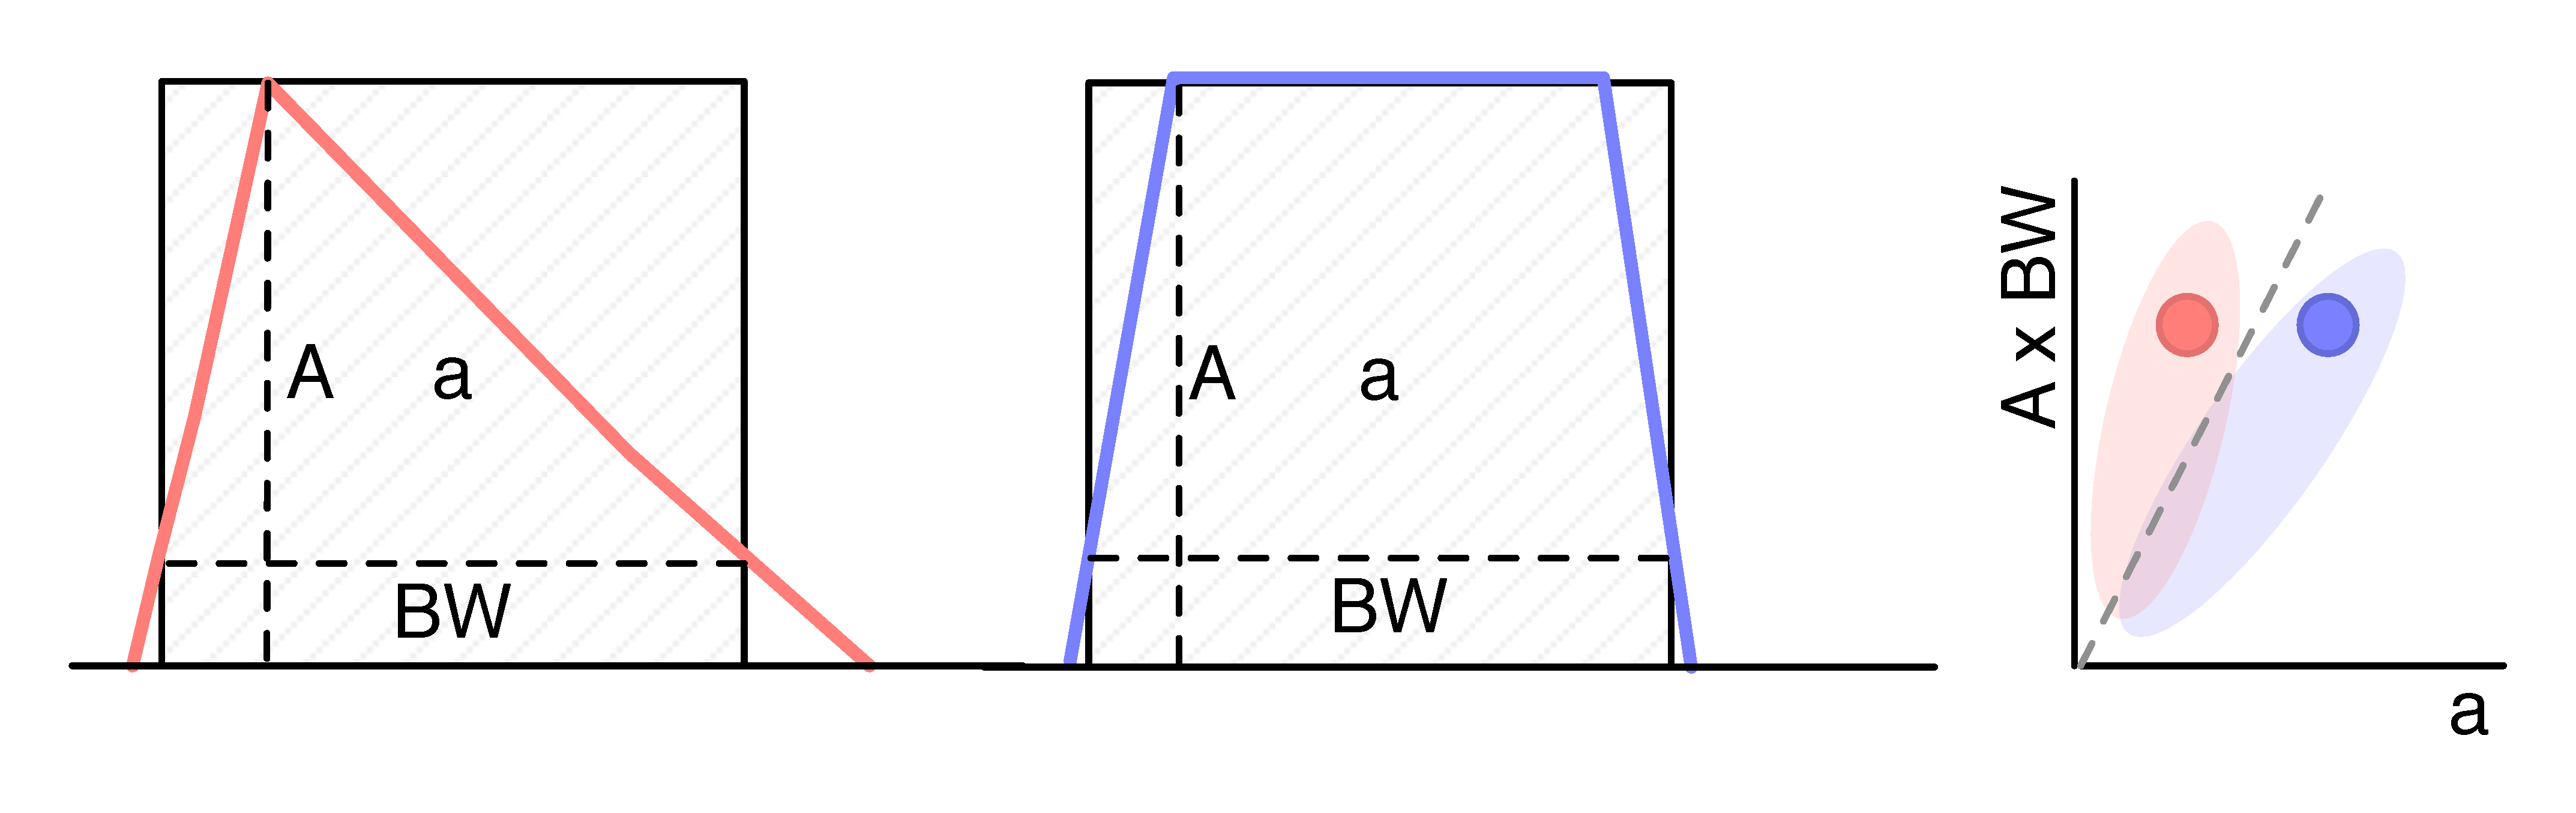
\includegraphics[width=0.9\textwidth]{05_current_monitoring/plots/formfac1}
\caption{Form Factor is the ratio between the measured area ($a$) and the calculated area ($A\times BW$) of the pulse. The calculated area is significantly larger than the measured area for a triangular triangular pulse, but less so for the rectangular one. The red and blue dot in the right plot are the value entries of the two pulses shown. The red and blue oval shapes depict the regions for the values expected from triangular and rectangular pulses. By carefully choosing the linear qualifier (dashed line) and taking only the entries below the cut rectangular pulses can be identified.}
\label{fig:formfac1}
\end{figure}

%Every parameter set is saved into a histogram after analysis.  The falling slope is not even a physical quantity, but as will be shown later, can improve the identification. 


%\subsection{Real-time pulse shape analysis algorithm}
%\clearpage
\section{Applications}
\label{sec:applications}

The FPGA firmware is designed for systems instrumented with CIVIDEC amplifiers and CIVIDEC sVCD diamond detectors. Three applications are available: \emph{Spectroscopy}, \emph{Pulse Shape Analysis} and \emph{Counter}, each optimised for a specific task. Their capabilities are described below. The firmware runs in ROSY, a readout system produced by CIVIDEC.

\begin{description}
\item[Spectroscopy] is a tool for measuring energy spectra of radioactive sources. It is used in combination with the CIVIDEC Cx spectroscopic charge amplifier. The signal from the charge amplifier is analysed in real time. The FPGA measures the maximum amplitude of the signal. The amplitude value is ready at the end of the pulse and is stored in the amplitude histogram. Immediately after, the analysis is reset and the system is ready for a new acquisition. Upon request from the software, the histogram is read out, during which the analysis is paused. In addition to the histogram building, the firmware can also store raw pulse waveforms, which can be then read out by the software. The maximum allowed throughput is 1~million counts per second.

\item[Pulse Shape Analysis] is a tool for measuring energy spectra of radioactive sources, with an additional feature. It can identify the type of radiation detected by the diamond detector. By means of the pulse analysis it can subtract the background radiation and only measure the signals from the defined radiation source. It is used in combination with the CIVIDEC C2 fast current amplifier. The firmware receives a current pulse from the detector and digitises it. The pulse is then analysed and parametrised. The analysis module measures its maximum amplitude, full width at half maximum (FWHM), baseline amplitude, falling slope and its area. Then it compares the obtained pulse parameters with the qualifiers set by the software and determines what type of radiation hit the diamond detector. Depending on the qualifiers, the pulse can either be \emph{accepted} or \emph{rejected}. The firmware then stores the parameters of the analysed pulse into histograms. Two histograms exist for each parameter: one for all pulses and one for accepted pulses. In addition, there is one 2D histogram (a scatter plot), which can plot two parameters one with respect to the other. Upon request from the software, all histograms are read out, during which the analysis is paused. The maximum allowed throughput is 1~million counts per second.

\item[Counter] is a tool that measures the count rate and the mean time during counts. It is used in combination with the CIVIDEC Cx, C6 or C2 amplifier. It contains one histogram which holds the information about the mean time during counts. The counter is operational also during the readout of the histogram. The highest counting rate with enabled histogram writing is 3$\times10^7~s^{-1}$.
 
\end{description}



\section{Description of the firmware}
The applications are built on top of the Picotech platform. The base code handles the communication between the software and the hardware. Furthermore, it provides the interface to the ADC data, the input/output registers and the USB data transfer. The applications have a set of modules that handle the data input and output and a module for signal analysis (see figure~\ref{fig:application}).. The data handling modules are very similar in all the applications to ensure compatibility of the communication between software and firmware and the readout data format. The analysis module, however, is different from one application to the other. The data handling layer is the same for all applications and consists of the final state machine (FSM), the histogram builder, the raw signal handler, the USB FIFO buffer and the register array.

The firmware is written entirely in VHDL. The diagram in figure~\ref{fig:application} shows the module architecture. The ADC provides the module with 32 digitised signal samples every clock cycle (6.4~ns). The signal is routed directly to the pulse analyser and into the raw signal handler. The analyser outputs are connected to the I/O registers and to histogram buffers. Both the histogram buffers and raw signal buffers are connected to the USB FIFO through a multiplexor. The firmware communication to the controller is done via input/output (I/O) registers (control and status registers, counters) and serially via USB (histogram data, waveforms). 


\begin{figure}[!t]
\centering
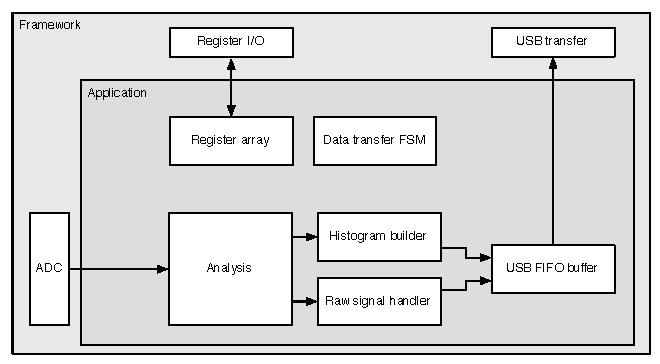
\includegraphics[width=0.9\textwidth]{05_current_monitoring/plots/application}
\caption{Firmware design structure}
\label{fig:application}
\end{figure}


\subsection{Design constraints}
\begin{description}
\item[Speed] The ADC provides 32 8-bit samples on every 6.4~ns clock cycle. It is not possible to e.g. sum all 32 values in a single cycle, because the summation takes too long to complete. This is why the summation has to be pipelined and carried out in three cycles. This adds up to the analysis duration, which in turn decreases the maximum pulse rate.
\item[Firmware size] The PSA application makes use of a number of FIFO and RAM buffers to store the pulse waveforms and histograms. 48 32k block RAM modules have been used for the implementation, maxing out the available block RAM memory space on this FPGA. The analysis algorithm also takes up a significant portion of the FPGA. Many of the operations are carried out on 256-bit long numbers received from the ADC, which quickly fills up the available logic. This is also why the place and route procedure takes a long time.
\item[Power consumption] The reduction of the power consumption is not crucial for the intended applications.
\end{description}


%=====================================================
\subsection{Analysis module}
\label{subsec:algorithm}
This module is different for different applications. The Pulse Shape Analysis (PSA) application has the most complex module design. The spectroscopy application only uses a small part of that design and the Counter application an even smaller one.


\begin{figure}[!t]
\centering
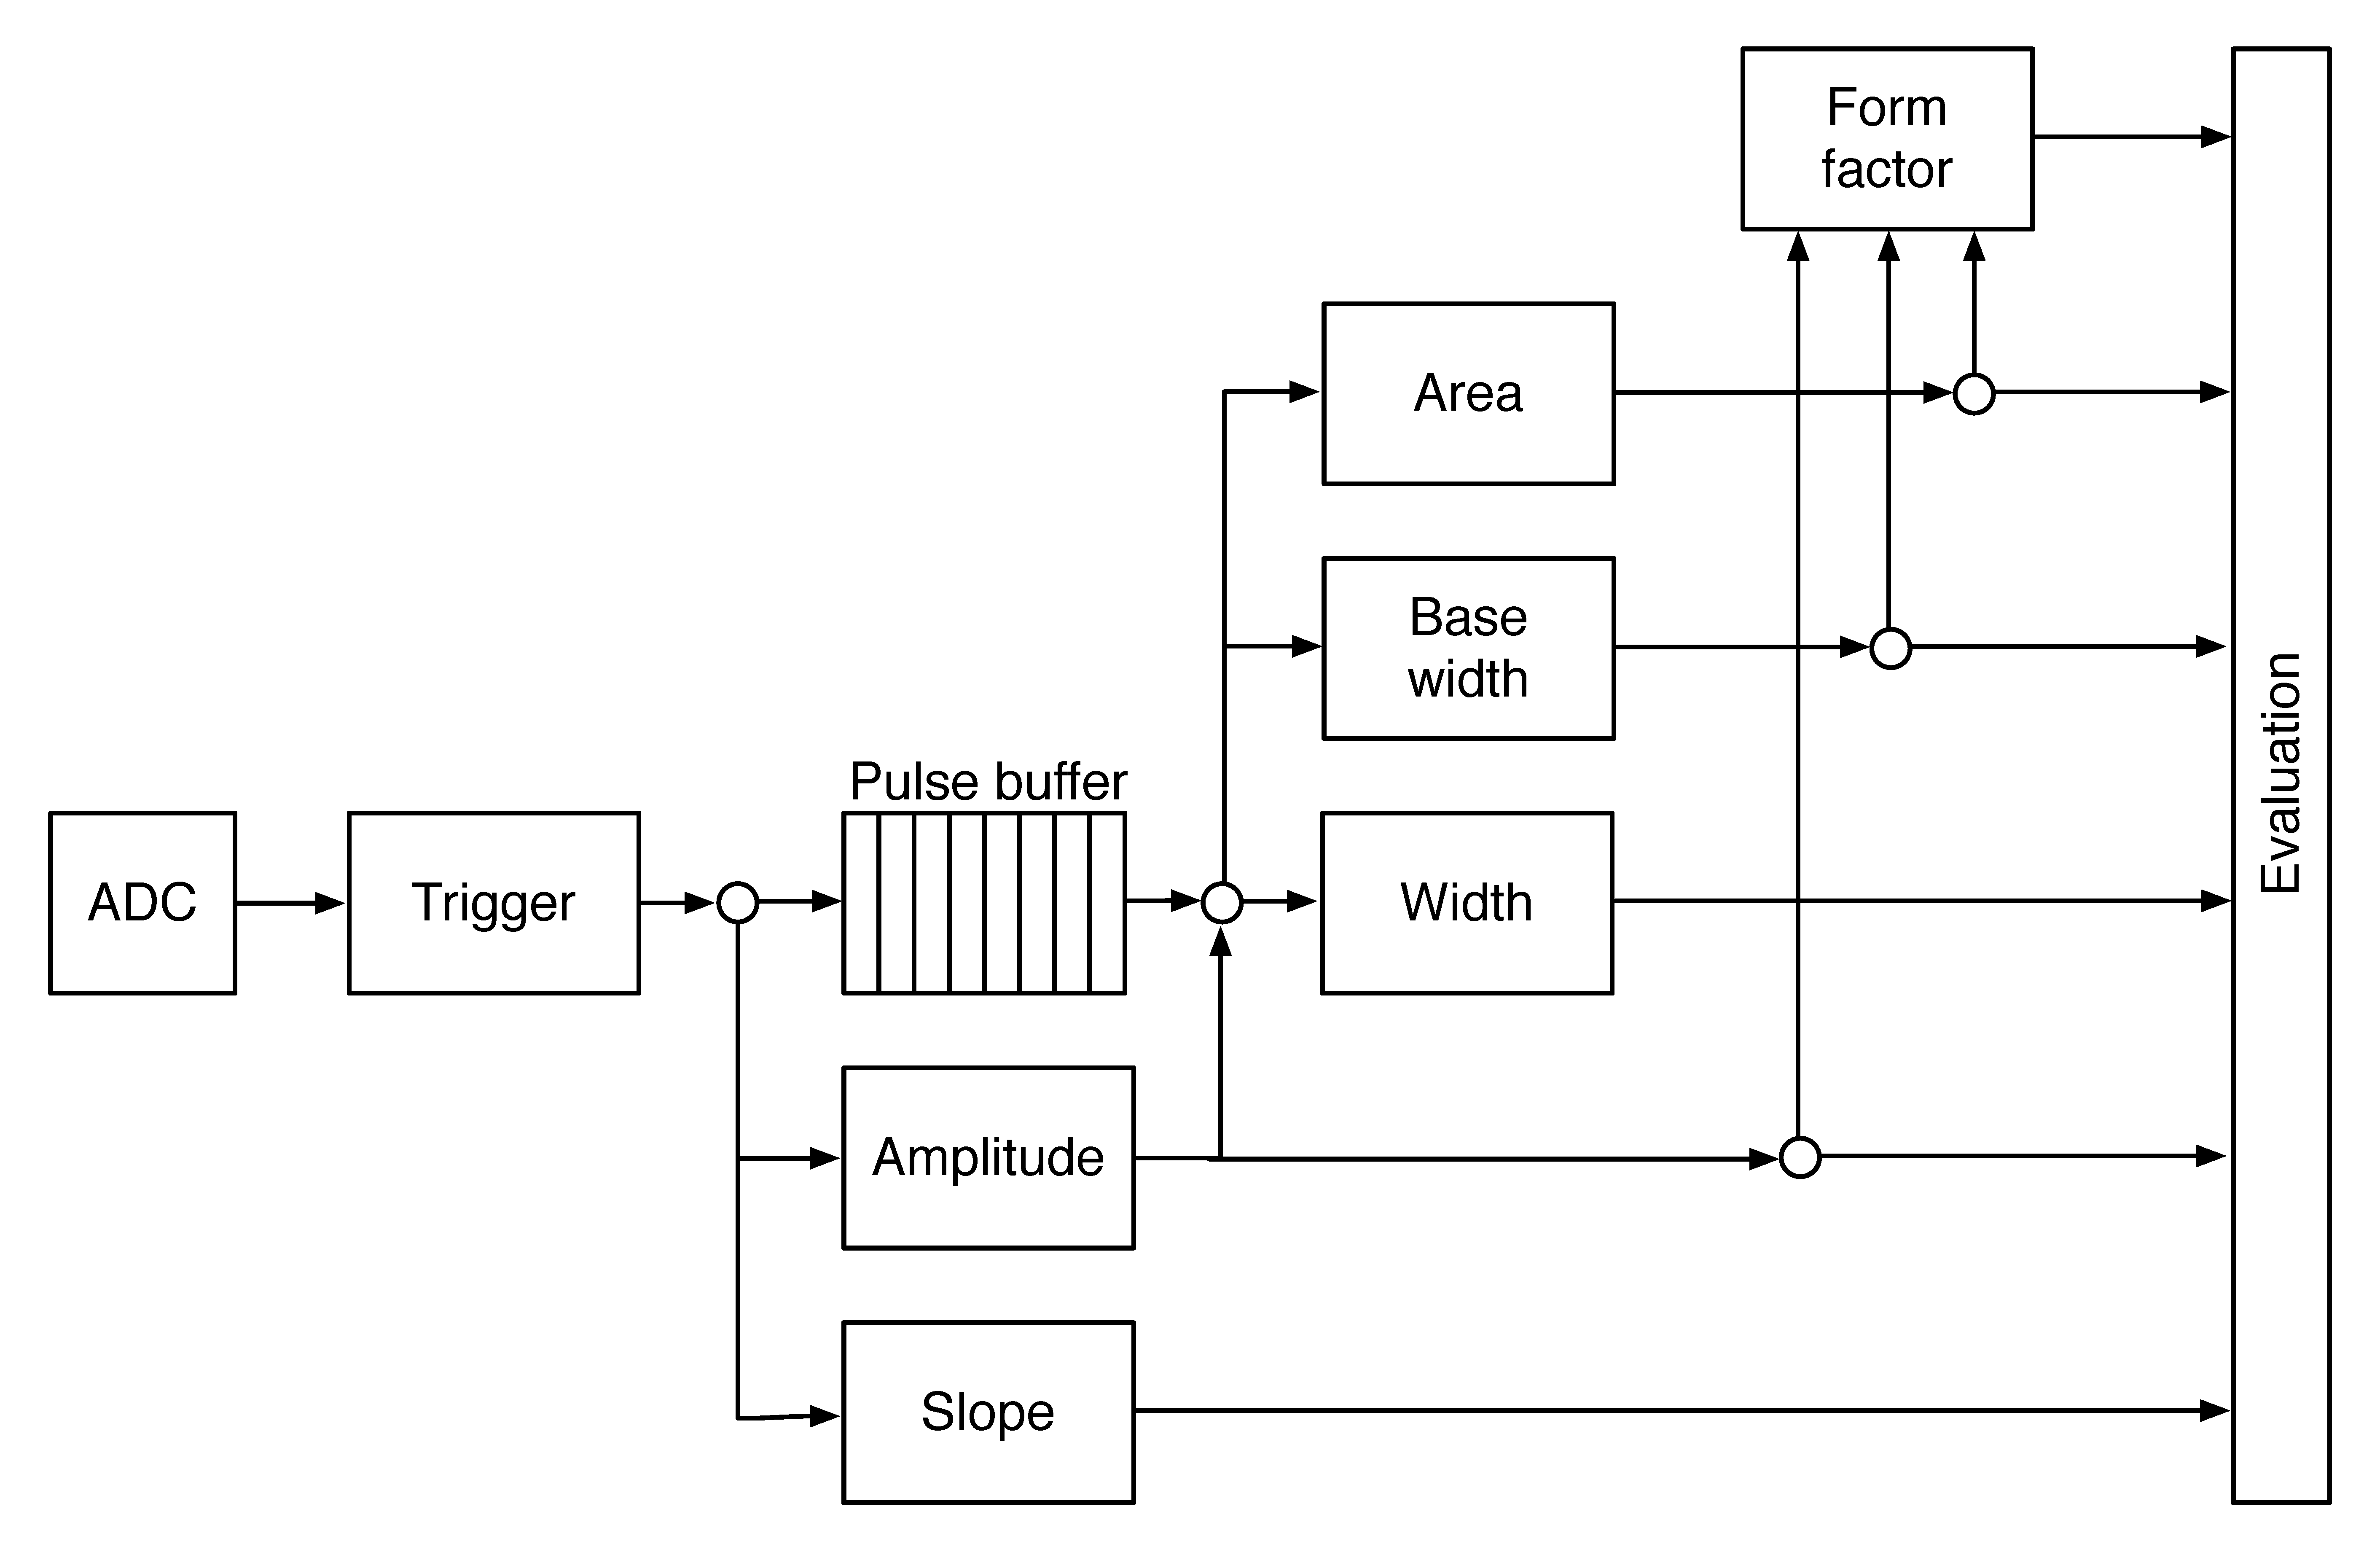
\includegraphics[width=0.9\textwidth]{05_current_monitoring/plots/analysis1}
\caption{Code design plan}
\label{fig:architecture}
\end{figure}

The analysis (or parametrisation) is carried out in several steps, as shown in figure~\ref{fig:architecture}. The triggering block starts the readout upon signal threshold crossing. The maximum slope of the falling edge is observed. The Amplitude block calculates the pulse height and retains the maximum amplitude while pushing the signal into the pulse buffer. Then the whole pulse is clocked out of the buffer while its FWHM, baseline width and area are measured. Finally, the Form factor is calculated. At the end the Evaluation block takes in all the parametrised information and classifies the pulse according to user-defined cuts. 

%Figure~\ref{fig:pulseana} shows the timing of the data flow within the block. All submodules are described in detail in the following subsections. The waveform in figure~\ref{fig:waveform1} is a simplified representation of the pulse analysis process. The logic bits show which modules within the PSA are active at which stage of the analysis.
\begin{description}
\item[Triggering] module handles signal polarity swapping, triggering on threshold and defining the trigger window. The real-time processing algorithm allows for a positive or an inverted input signal. However, the PSA only handles positive-polarity pulses. Therefore a negative signal is swapped in the \textit{triggering} block. Signal analysis and readout are then triggered when the signal crosses a user-defined threshold. In addition, the signal has to be over the threshold for a defined number of samples. This is to avoid triggering on noise spikes.
A double clock cycle delay is used on the signal to make sure that the recorded signal window will include the rising edge of the pulse as well as some baseline before it. A \textit{trigger active} signal marks a window that contains the whole pulse including some baseline signal before and after it. 
The trigger can be vetoed by three signals: if the pulse analysis is still taking place, if the input signal exceeds the maximum voltage range or if the data transfer FSM is pausing the analysis due to data transfer to the controller.

%\subsubsection{Baseline producer}
%\label{subsub:base}
%This module has two functionalities. It carries out baseline noise filtering and it produces a baseline signal during a pulse. The filtering is implemented as a moving average of four data points. User can choose which four points to use: every first, second, third or fourth sample.
%
%Baseline signal during a pulse is used to calculate pulse height. It is produced by re-playing the last 64 data points of the baseline in a loop (an example shown in figure~\ref{fig:pulsepars}). It is implemented as a double register which replaces the real signal during the trigger window.


\item[Amplitude] block calculates the pulse height from the difference between the pulse and the baseline. It also finds the position of the maximum amplitude within the clock cycle. It receives 32 8-bit samples from the triggering block every clock cycle. Time delays in the logic prevent it to find the maximum value of the 32 samples within one clock cycle (6.4~ns). Therefore the decision logic has been pipelined in three stages, which means that the final maximum value is ready three clock cycles after the end of the pulse.
\item[Pulse buffer] is a FIFO that stores the signal while its amplitude is being measured. At the end of the pulse the FIFO is read out so that the remaining measurements can take place. 

\item[Width] block uses the maximum amplitude to determine the \emph{half-maximum} and to measure the FWHM. To do so, it counts the samples that are above the half-maximum amplitude. However, this method might also count high enough noise spikes before or after the pulse. Hence an improved method, which ``cleans'' the measurement of unintentional additional noise, has been implemented. It is described in section~\ref{sec:vecclean}.
\item[Baseline width] block is the same as the Width block, but it measures the width either at 50~\%, 25~\%, 12.5~\% or 6.25~\%, depending on the setting in the register. It also makes use of the special method described in~\ref{sec:vecclean} to avoid overestimations due to including noise in the measurement.
\item[Area] block measures the pulse area by summing up the amplitude values of the samples in the pulse. The boundaries of the summation are defined with the crossing of the amplitude above a certain threshold. Only the samples between those boundaries are summed up. The boundaries can be set at  50~\%, 25~\%, 12.5~\% or 6.25~\% of the maximum amplitude of the pulse. The area measurement makes use of the same routine as the FWHM and Baseline width block to remove the potential outlying samples.

\item[Falling slope] block measures the highest negative difference between amplitudes of two adjacent samples, thus getting the maximum negative slope of the pulse. It is an experimental routine, only used for academic purposes.
\item[Form factor] block is used as a special qualifier for particle identification. It compares the weighted measured area of the pulse with its weighted calculated ``form'', which is defined as the multiplication of the measured amplitude and baseline width. The equation is as follows:
\begin{equation}
\label{eq:formfactor1}
x\cdot a - y \cdot A \cdot BW \geq 0,
\end{equation}
where $a$ is the measured area, $A$ is the amplitude, $BW$ is the baseline width and $x$ and $y$ the weighting factors for the measured and calculated area, respectively. The output of the block is the boolean result of this equation.
\item[Evaluation] block takes in all the parameters from the analysis blocks and compares them against the user-defined qualifiers. If the parameters are within the bounds, the pulse is accepted, otherwise it is rejected. The corresponding counters within the block are incremented.

\end{description}


\subsection{Area and width measurement}
\label{sec:vecclean}
The routine for measuring pulse area and width must have a specific algorithm implemented to carry out the measurements correctly. The core point is that the routine precisely defines the edges of a pulse. It does so by means of \emph{vector cleaning}, presented in figure~\ref{fig:samplepulse}. An important input, beside the ADC data and the measurement threshold, is the position of the sample with the highest amplitude. 

The signal arrives from the ADC as a set of 32 8-bit samples every every clock cycle with a period of 6.4~ns. All 32 samples are compared against the width measurement threshold. If a sample value is equal or higher than this threshold, a binary 1 is set in a 32-bit \emph{vector} on the position corresponding to the position of the sample in the incoming ADC data set. The resulting vector might also include some noise at the edges of the pulse, depending on the height of the width measurement threshold. The old routine simply counts the binary ones in this vector to get the pulse width. This works well for measuring the FWHM because the threshold was high. However, for width measurements at 25~\%, 12.5~\% or 6.25~\% of the pulse height this might already become a problem, because the noise might be counted in as well. This is why the new routine cleans the outliers in this vector before counting the remaining ones in the clean vector. 

\begin{figure}[!t]
\centering
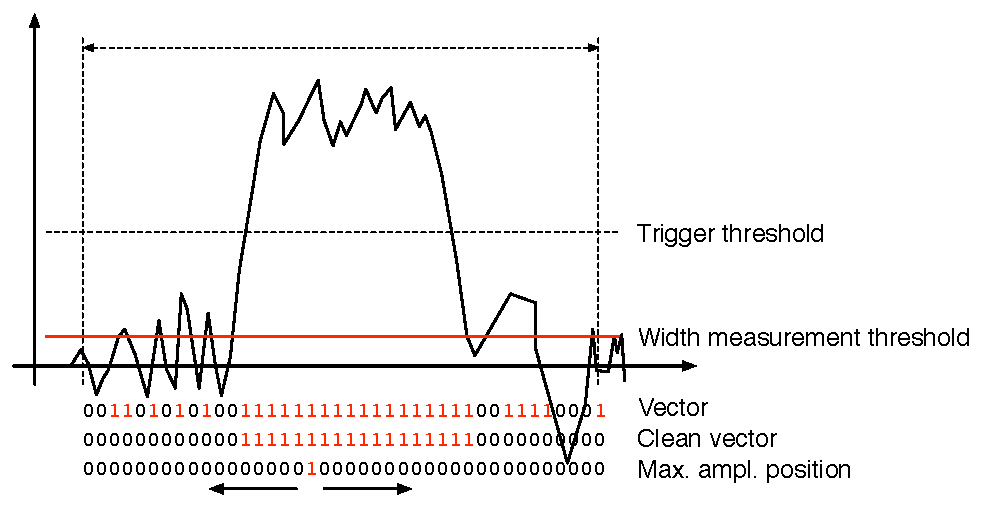
\includegraphics[width=0.7\textwidth]{05_current_monitoring/plots/pulse1}
\caption{A sample pulse. The first vector shows which samples are above the width measurement height. The second vector is a clean vector. The third line shows the position of the maximum amplitude. The vector cleaning algorithm starts from the maximum amplitude and continues in both ways along the vector.}
\label{fig:samplepulse}
\end{figure}

The routine starts from the position of the maximum height. It follows the vector in both ways and finds the first falling edge (0 at this position and 1 at the previous one). From there on it rewrites any binary 1 with a binary 0. The resulting clean vector only has one bunched set of binary ones which are summed, yielding a precise pulse width. The area measurement is similar - it only integrates over the samples marked in the clean vector. Both measurement routines, for area and for width, are implemented separately so that the area routine can have a different threshold set.

This section explains how the algorithm is designed. First, the idea for it was tested using Excel and was only afterwards ported to the VHDL. The underlying algorithm first cleans the vector. Then it passes the cleaned vector either to the width or area measurement (see figures~\ref{fig:width} and \ref{fig:area}). The width measurement module only sums the ones in the vector whereas the area measurement module sums the data samples marked by the cleaned vector. Both modules issue a \emph{valid} signal when they finish the measurement.

\begin{figure}[!t]
\centering
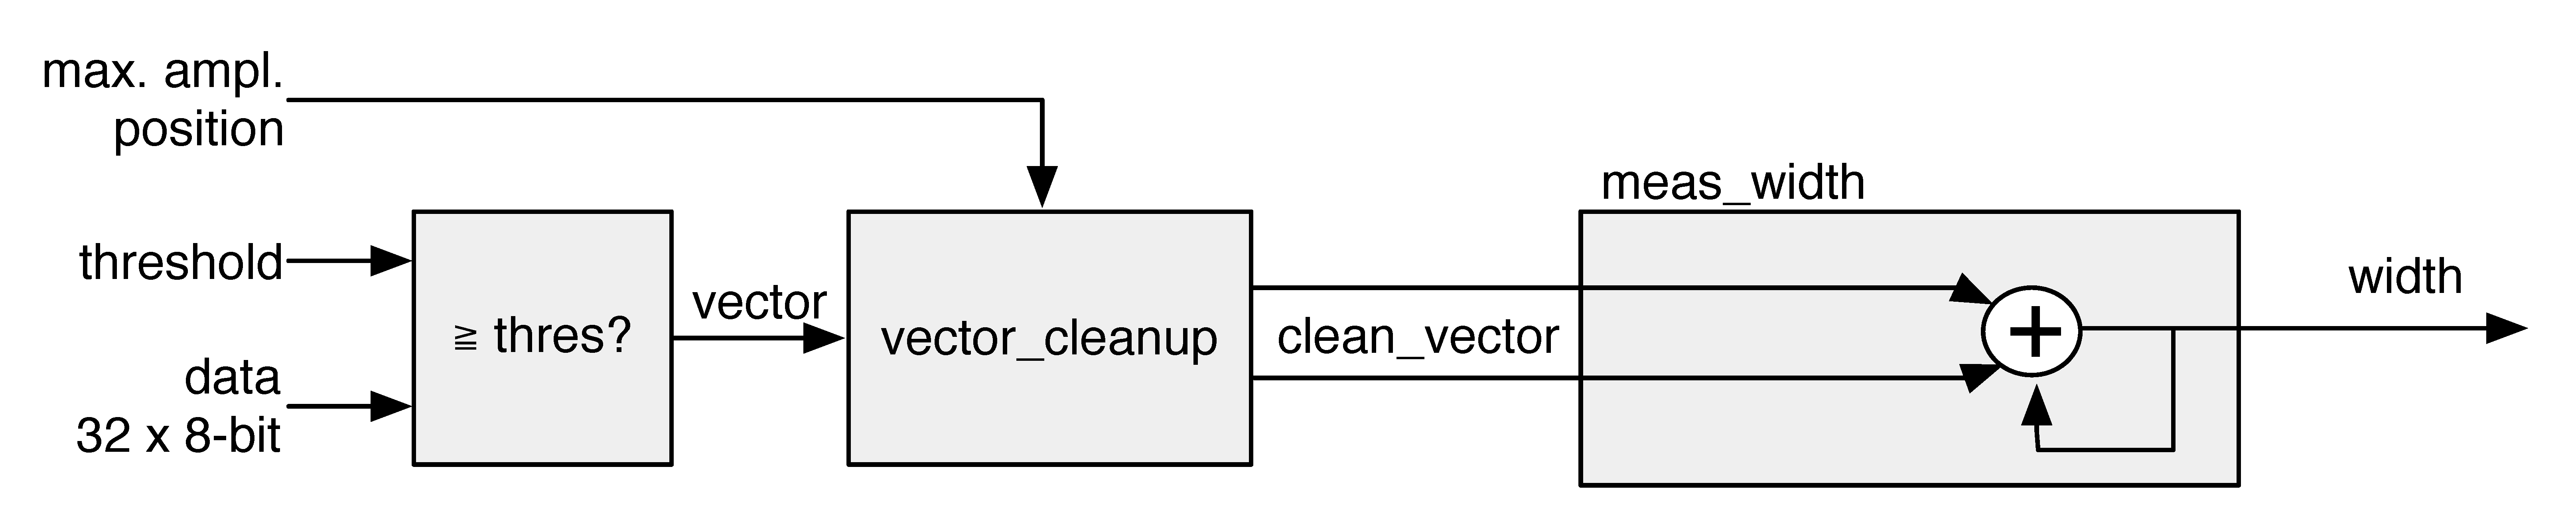
\includegraphics[width=0.95\textwidth]{05_current_monitoring/plots/width2}  \label{fig:width}
\caption{This block counts the remaining binary ones in the clean vectors and outputs this value as the pulse width.}
\end{figure}


\begin{figure}[!t]
\centering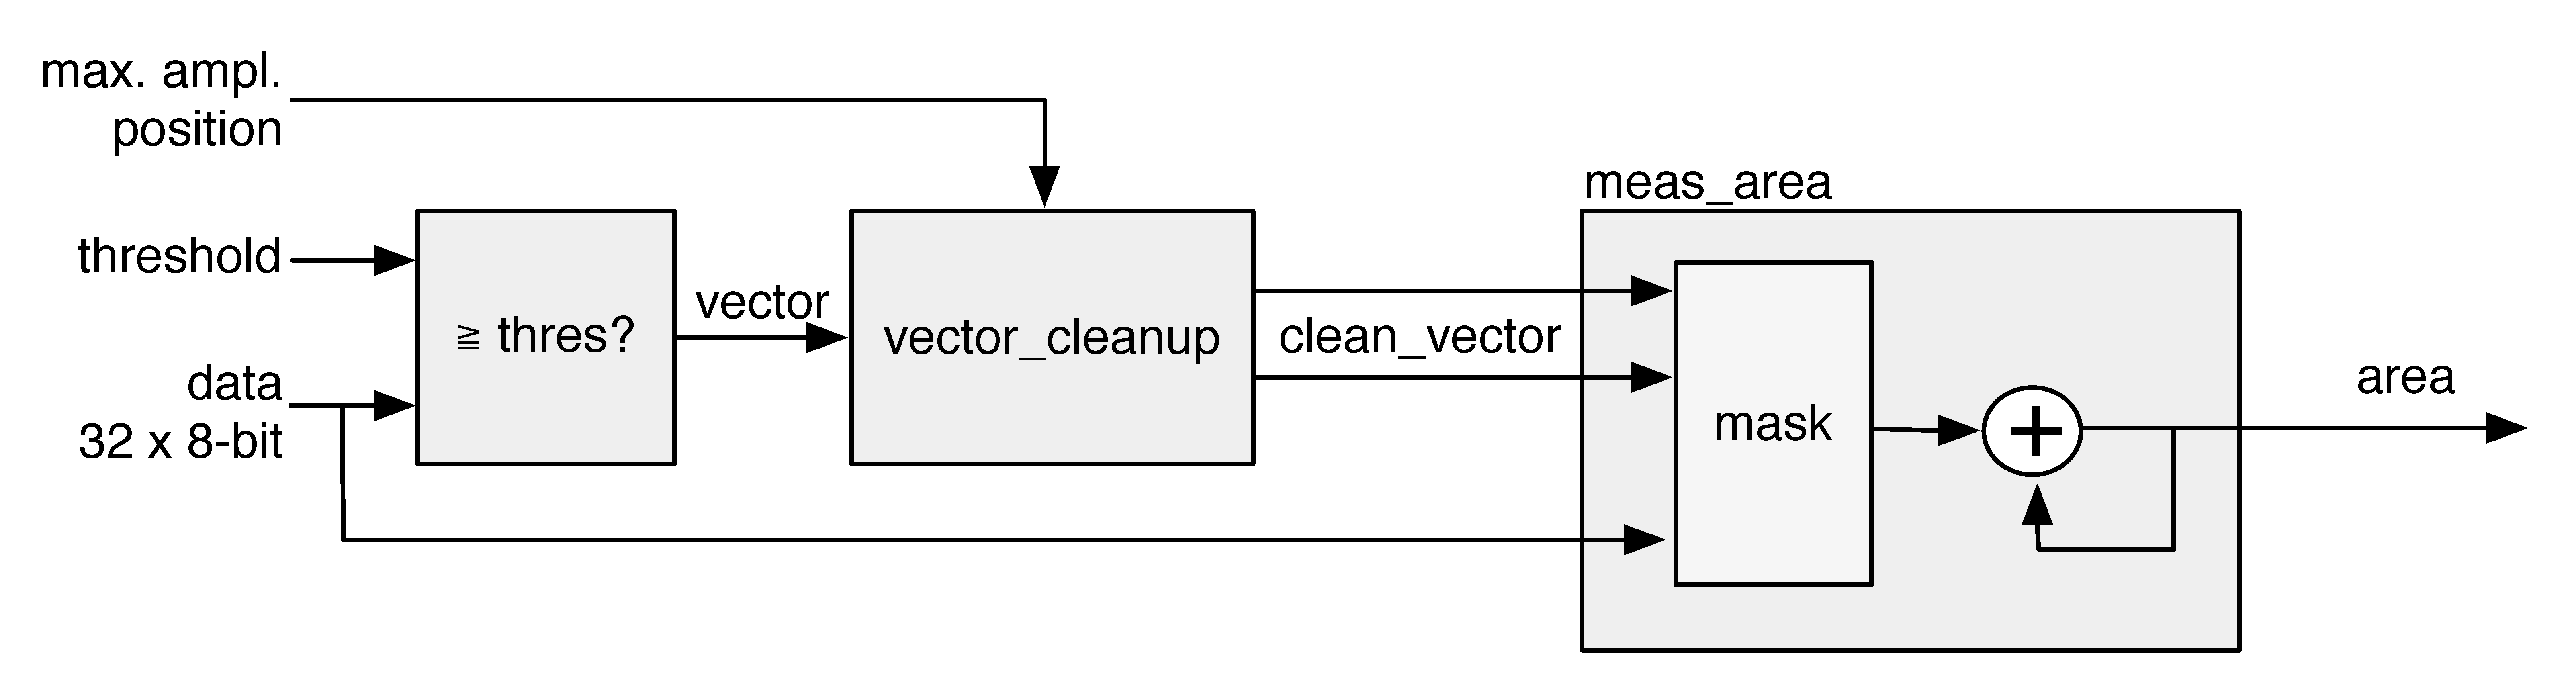
\includegraphics[width=0.95\textwidth]{05_current_monitoring/plots/area2}  \label{fig:area}
\caption{This block masks the input data with the clean vector and sums the remaining samples.}
\end{figure}


 
\subsubsection{Vector cleaning}
This is the most important block. Its inputs are: \emph{vector, parsing active, position of the max. amplitude (PA) and its delay (DA)}. PA is a 32-bit binary number that shows the position of the sample with the maximum amplitude within the data block whereas the DA tells us how many clock cycles after the start of the parsing this PA block is.
\begin{figure}[!t]
\centering
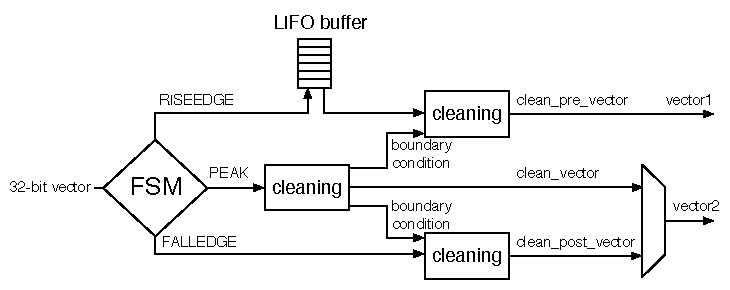
\includegraphics[width=0.9\textwidth]{05_current_monitoring/plots/vector_clean}
\caption{Vector cleaning routine outputs two vectors - one forward in time and one back in time from the peak of the pulse.}
\label{fig:routine}
\end{figure}
The vector cleaning module is designed as a final state machine (FSM) with the states IDLE, RISEEDGE, PEAK, FALLEDGE and READY.  The FSM is idle until it receives the \emph{active} signal from the external module, marking that the vector parsing has commenced. It switches to RISEEDGE, which starts two procedures: 1) it fills the vector of the pulse's rising edge into a last-in-first-out (LIFO) buffer and 2) counts down from the DA value. When this counter reaches 0, the FSM changes its state to PEAK because the current vector on the input is the one containing the maximum amplitude. This data block is sent through the \emph{peak algorithm}, which cleans the vector. The FSM switches to FALLEDGE state. Now both the previously buffered vector of the rising edge and current vector of the falling edge go through the \emph{pre- and post- algorithm} where they are cleaned, but they get their boundary conditions from the \emph{peak algorithm}. The output of this module is therefore two cleaned vectors in parallel -- one forward in time and the other backwards.



\subsubsection{Algorithm}
The underlying algorithm is sequential - it carries out a logic operation on vector bit on position 0, uses the output of this operation for the operation on bit on position 1 and so on. This means that it has to carry out 32 logic operations per clock cycle. With each operation taking approximately 0.3~ns, the whole logic chain takes approximately 10~ns to complete. With only 6.4~ns per clock cycle, this means timing errors would occur. To fix the problem, a more complicated \emph{decimated algorithm} has been designed. It consists of two parallel logic chains. Each of the two only takes every second bit into account (chain one: 0, 2, 4 ..., 30. Chain two: 1, 3, 5 ..., 31). This makes the chains effectively 16 bits long. The algorithm is run on the two chains and the results are merged together at the end as shown in figure~\ref{fig:algobase}. This effectively reduces the number of sequential logic operations to around 18, which is within the timing constraints. 
%Nevertheless, to explain the algorithm, a non-decimated version will be shown first.
%This would need to be explained more in detail I guess...



\begin{figure}[!t]
\begin{tabular}{rr}
\subfloat{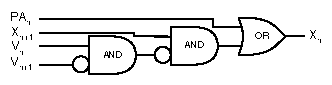
\includegraphics[width=0.47\textwidth]{05_current_monitoring/plots/logic1} \label{fig:logic1}} &
\subfloat{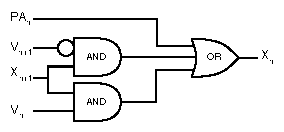
\includegraphics[width=0.47\textwidth]{05_current_monitoring/plots/logic2}  \label{fig:logic2}}
\end{tabular}
\caption{One logic step in the algorithm chain before and after Karnaugh minimisation.}
\end{figure}

\begin{figure}[!t]
\centering
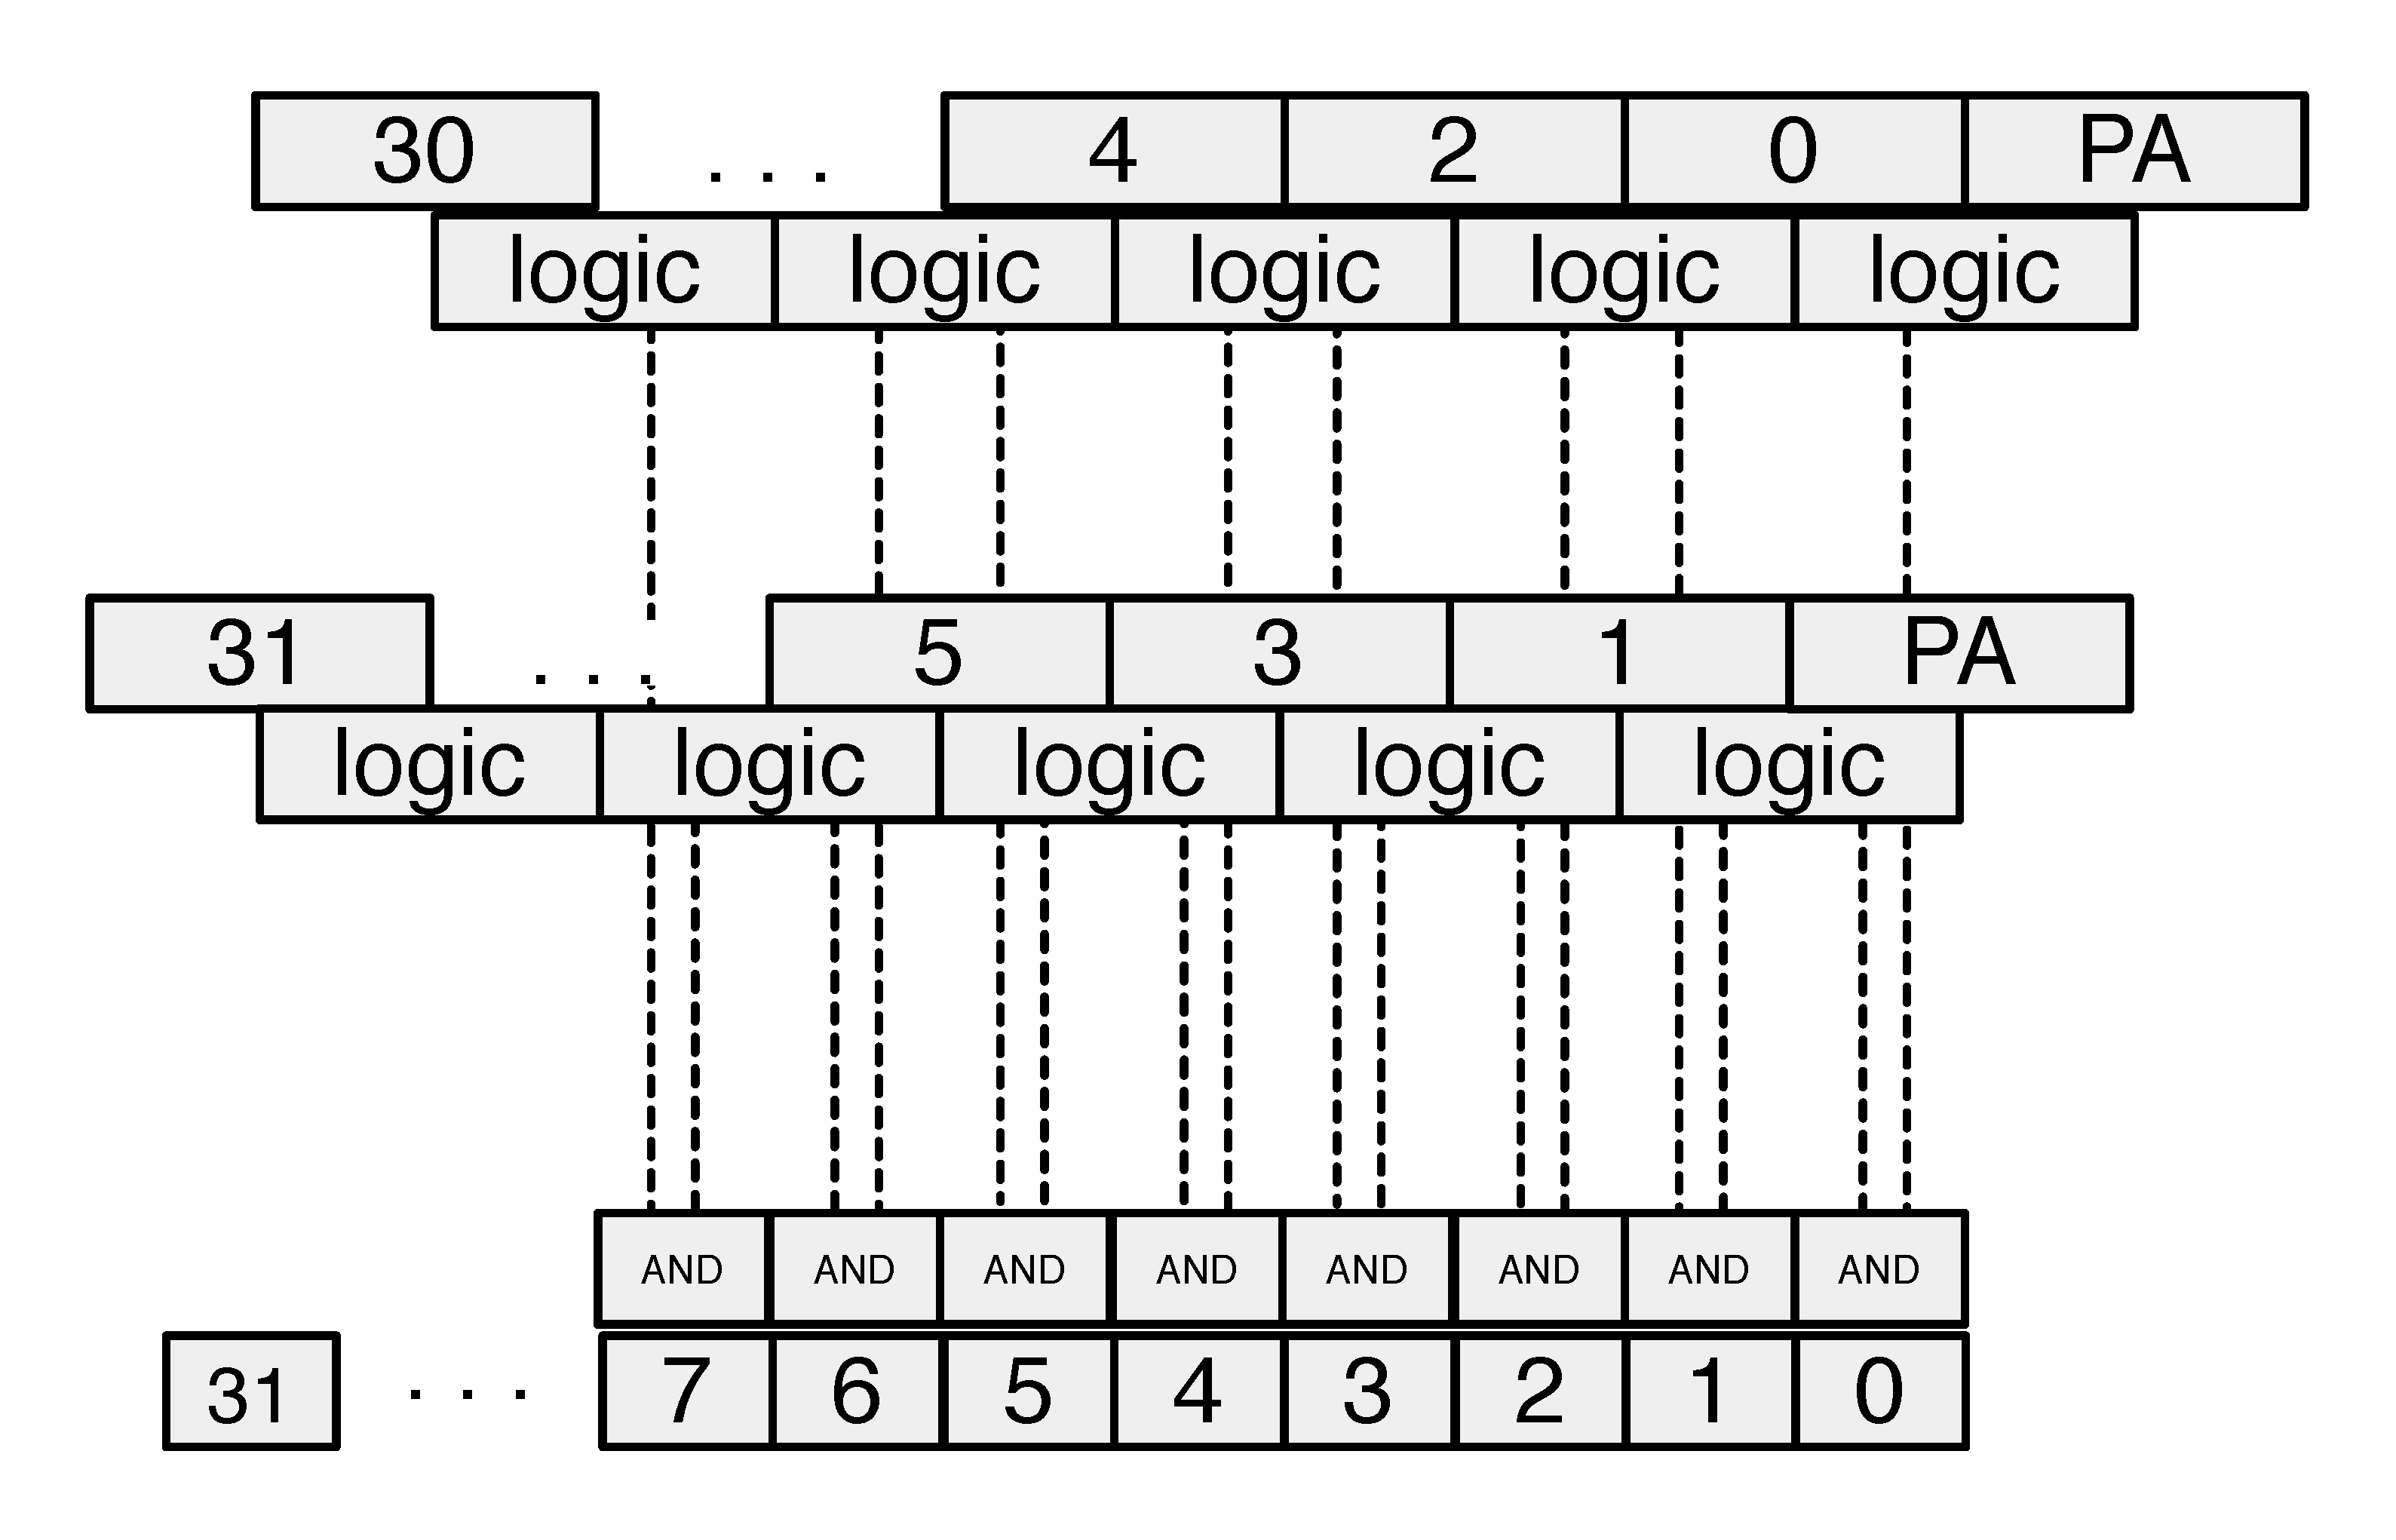
\includegraphics[width=0.7\textwidth]{05_current_monitoring/plots/algobase}
\caption{Vector is divided into two 16-bit logic chains. The algorithm logic is then run on the two chains separately. The results are then merged into one 32-bit clean vector by using a set of AND gates.}
\label{fig:algobase}
\end{figure}


\section{Control and data interface}
Communication between the device and the controller PC is done via the API functions provided by the producer. In addition, the API used by CIVIDEC has access to several extra functions. These allow the user to download a customised bitfile to the FPGA, access the I/O registers and use the USB data transfer.

\subsection{Software}
The software has been designed in C++ in several levels of abstraction. Figure~\ref{fig:controller} shows the structure of the classes. The classes Device, PSA and RawSignalHandler are there to make it easier to read and understand the controller code. In principle the PSfunctions can also be accessed directly by the controller, but for this the instruction sequences must be well known and understood. 

\begin{figure}[!t]
\centering
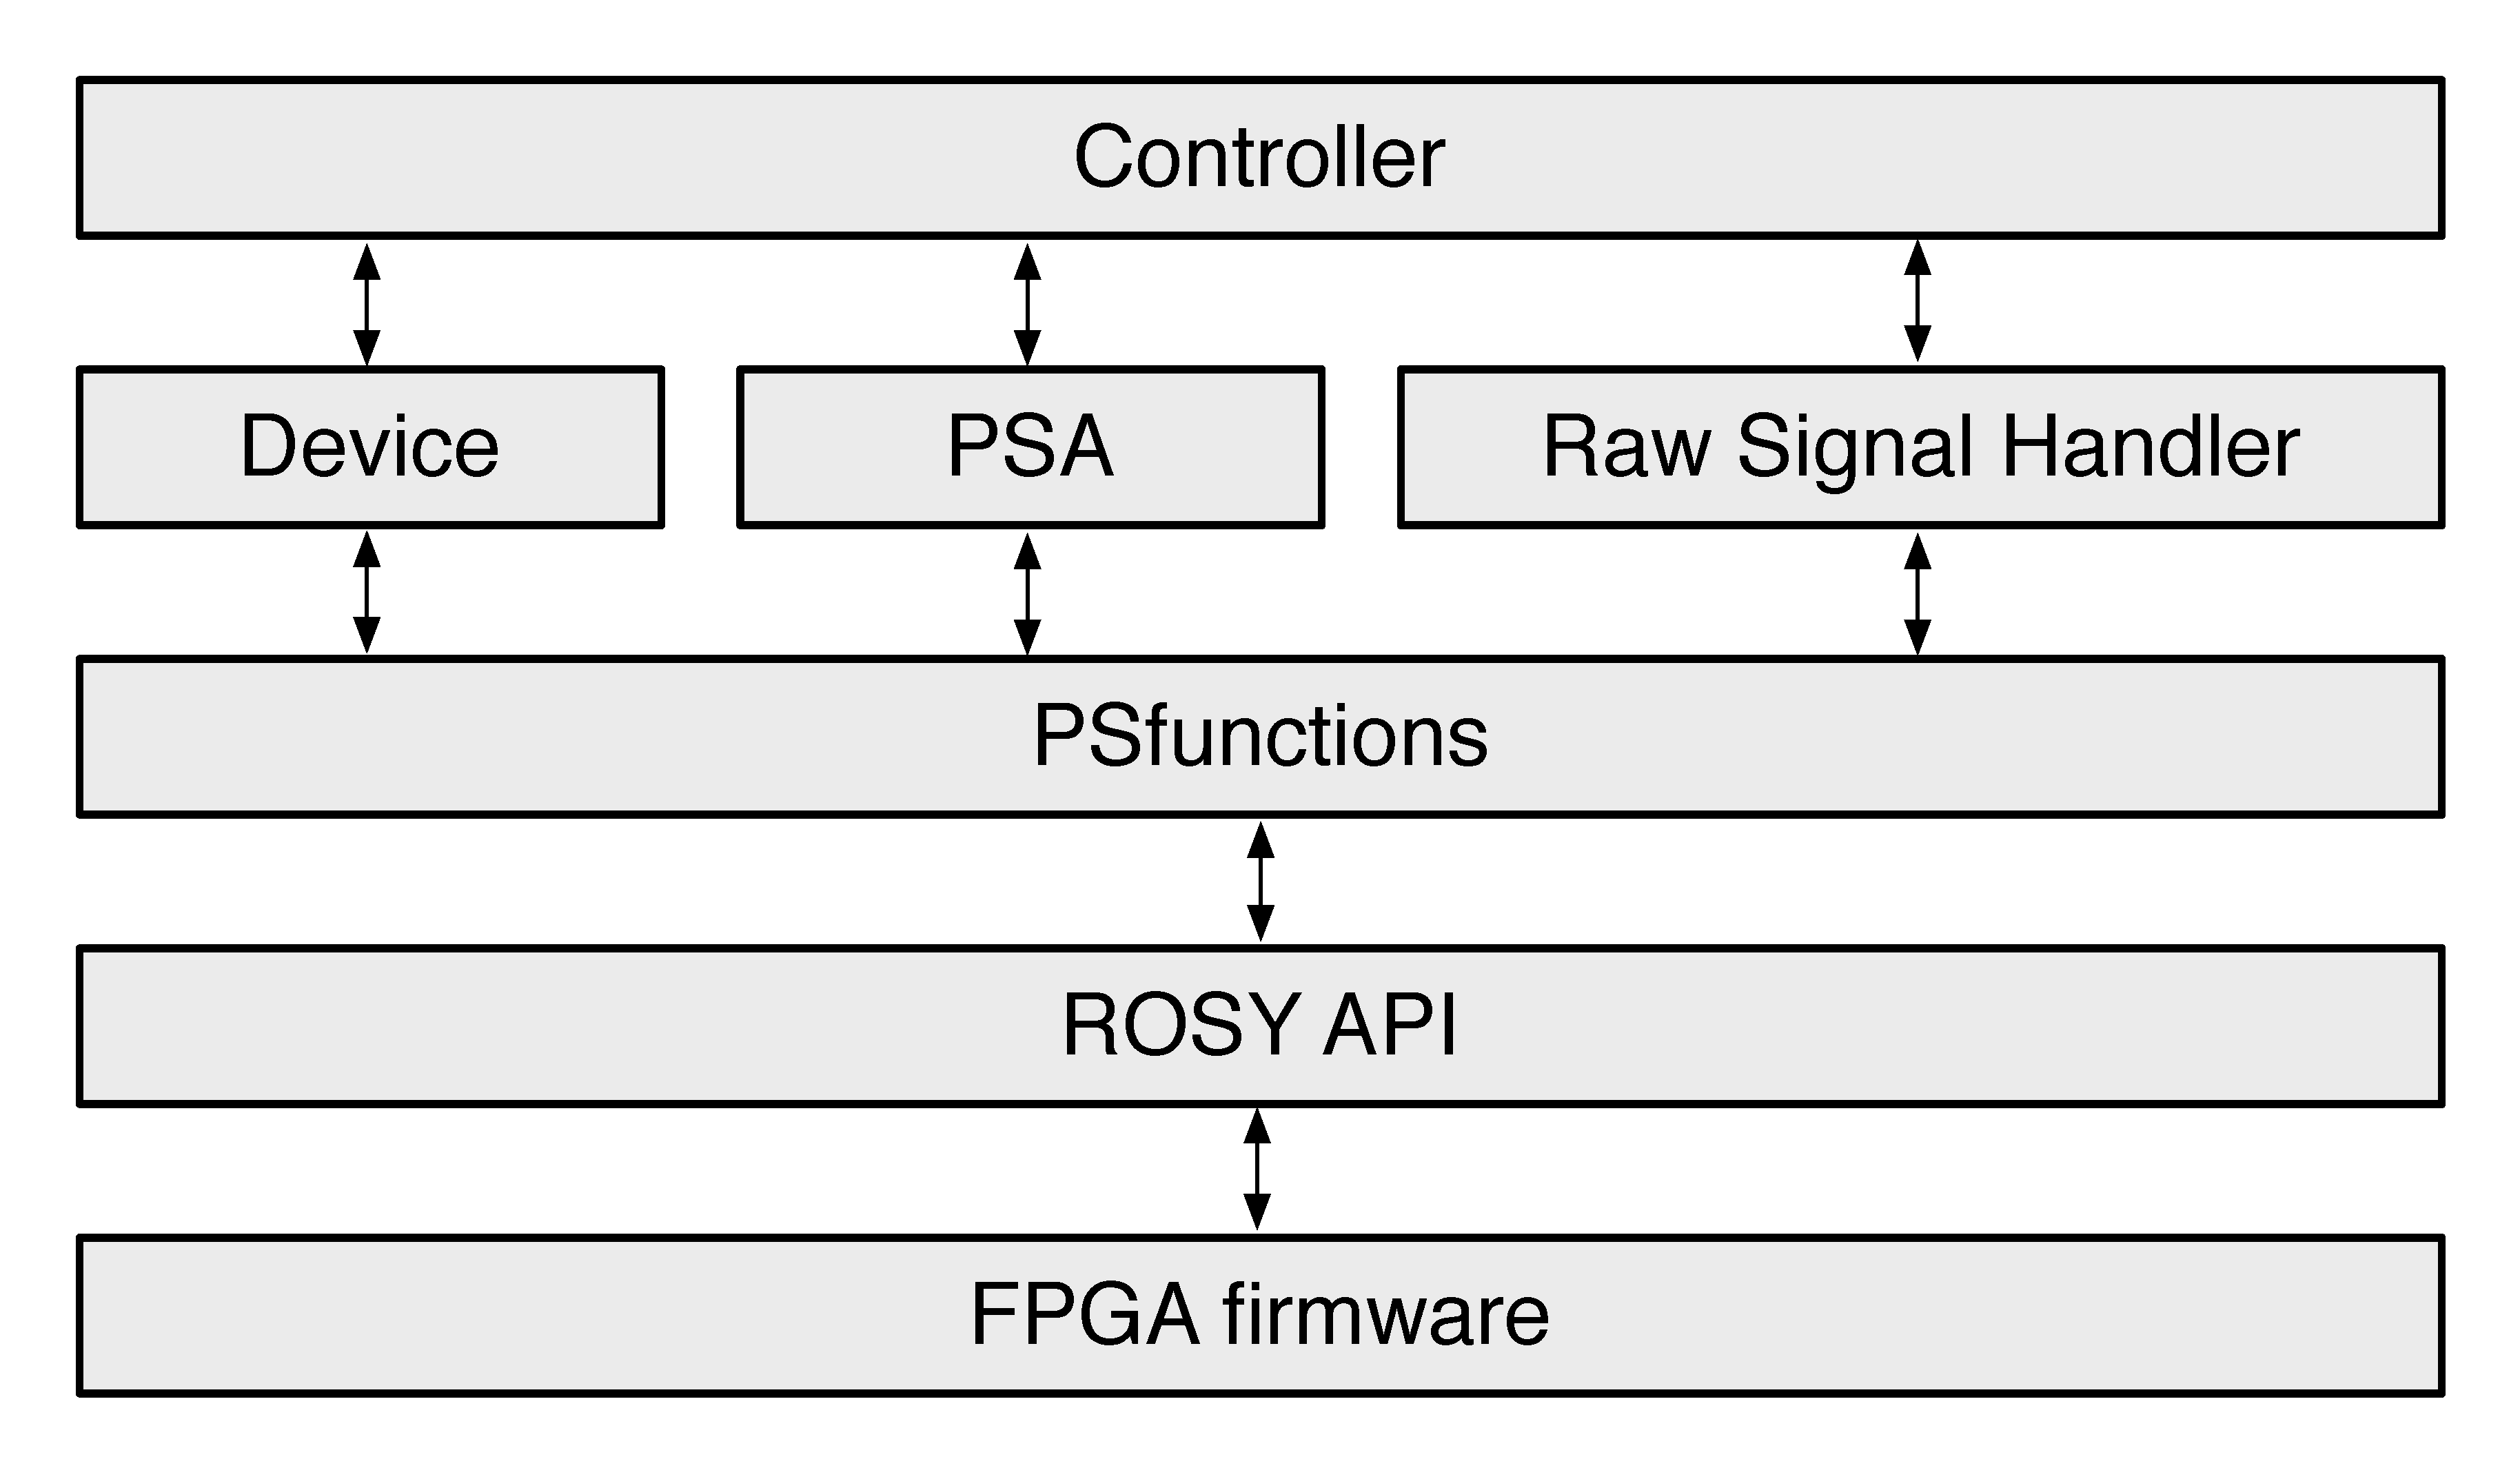
\includegraphics[width=0.6\textwidth]{05_current_monitoring/plots/controller}
\caption{Abstraction levels of the controller software}
\label{fig:controller}
\end{figure}

\subsection{Data readout}
The device records the data in two forms - as signal waveforms and as histograms of analysed pulse parameters. Both are available upon request from the controller. Only one of the two can be transferred via the USB line at a time. 
%The waveforms are read out as a series of 64 pulses whereas the histograms are 

The waveforms are saved into a FIFO buffer, which can hold up to 64 pulses of the length of $\sim$500~samples. The data format for each pulse is such that it starts with a header containing the pulse timestamp and the sequential number, continues with the data samples and ends with a header containing all the measured parameters (width, amplitude, area, fallling slope and form factor). When the FIFO is full, it issues a flag, which tells the controller that the data buffer is ready for readout. 

The histograms are implemented into the FPGA's Block RAM. Their size ranges from 256 to 4096 bins (an 8-bit or a 12-bit histogram, respectively), depending on the required histogram resolution. For instance, the width parameter is measured with a 0.2~ns resolution; the expected maximum pulse width is less than 20~ns. This yields the maximum range of 100 bins, making an 8-bit histogram sufficiently large. The same reasoning is applied to the amplitude measurement. In this case the maximum range is defined by the 8-bit resolution of the ADC. The area measurement, however, yields higher values and can therefore have a more refined binning (12-bit). Finally, a single 12-bit 2D histogram is included, with 6 bits for every axis. It is used as an online scatter plot for comparing one measured parameter to another. An example for it is a comparison of the width against the area, which can help the user determine the cuts that need to be applied to the measurement.




























% ---------------------------------------------------------------------------------------------------------------
%\clearpage
\section{Performance results}
\label{sec:perres}
% ---------------------------------------------------------------------------------------------------------------
The device has been tested in the lab using a pulse generator as well as several radioactive sources. The results show that: 1) the amplitude, area and width measurement are linear across all input ranges, 2) the highest rate of the PSA algorithm is $\sim5\times10^6$ pulses per second and 3) the lowest SNR where the algorithm still functions is $\sim$5.  

\begin{description}
\item[Trigger rate]
A pulse generator was used to verify the highest achievable rate at which the PSA still analyses every incoming pulse. The final state machine implemented in the pulse analysis module prevents the triggering block from issuing a trigger due to an incoming pulse if the previous analysis is still in ongoing. Given that all the pulses were of the same length, the analysis duration was always the same. When the time between the incoming pulses was shorter than the time of the analysis, the pulses were not analysed. Figure~\ref{fig:trigrate} shows the sharp decline in the percentage of the analysed pulses when reaching the rate of 5~MHz. Therefore the overall analysis duration for a 10~ns pulse is approximately 200~ns.

\begin{figure}[!t]
\centering
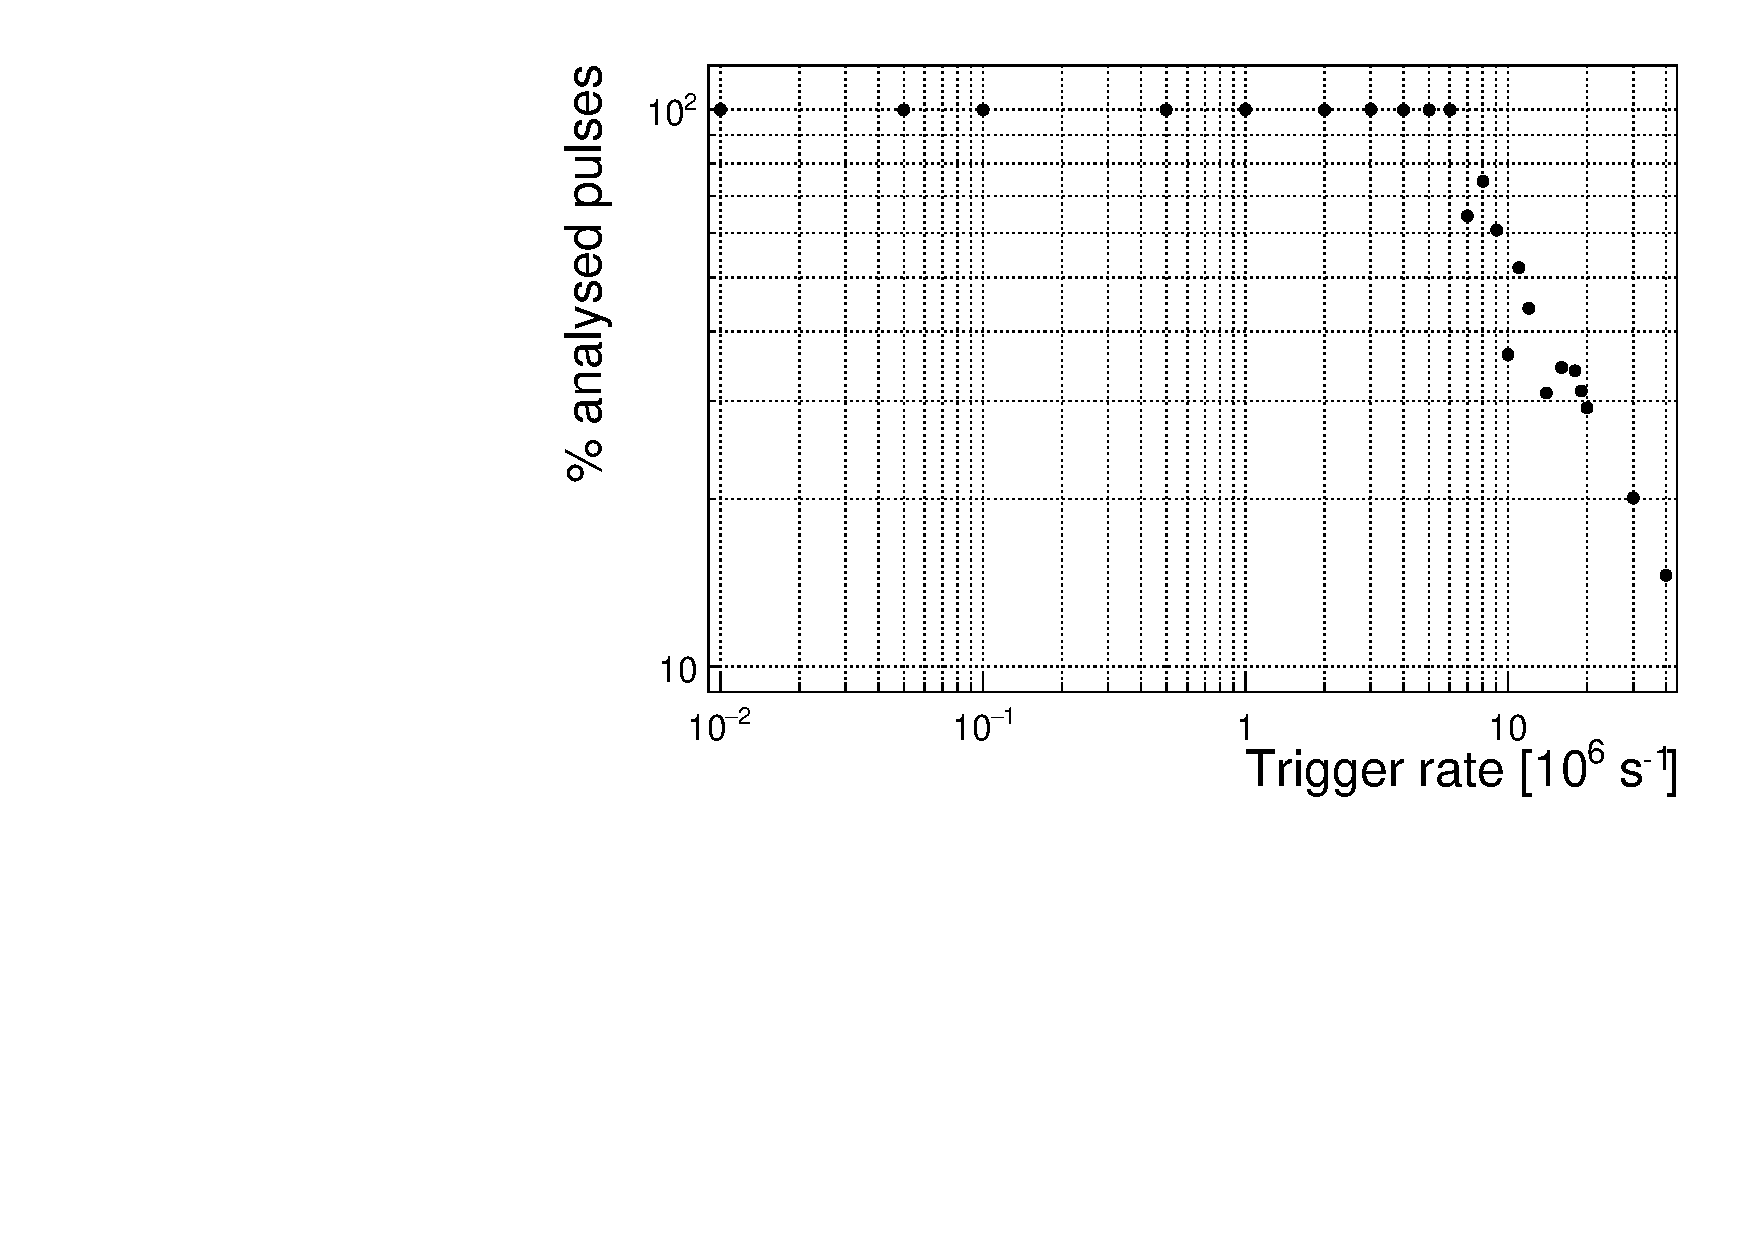
\includegraphics[width=0.8\textwidth]{../scripts/05_current_monitoring/PulseGenTests/plots/freq}
\caption{This figure shows the capability of the device to analyse all arriving pulses for a range of input frequencies. The highest achievable rate with zero lost pulses is $5\times10^6$~s$^{-1}$.}
\label{fig:trigrate}
\end{figure}

\item[Linearity]
A pulse generator was used to verify the linearity of the measurements across all input ranges. Pulse width and amplitude were varied and measured both with the oscilloscope and the PSA to check for non-linearities or inconsistencies in the PSA measurements. The resulting plots in figures~\ref{fif:ratioAmpl1} and~\ref{fig:ratioWidth1} show that the PSA measurements agree well with those from the oscilloscope. The major inconsistency is observed in the lower range of the plots. It stems from the fact that the bandwidth limit of the PSA is lower than that of the oscilloscope, which affects the pulse shape. Effectively, the PSA cannot measure the rectangular pulses of the width smaller than 2~ns.

\item[Stability]
The input pulse signal was superimposed with white noise generated by a noise generator with a variable gain. The mixed signal yielded pulses with an SNR ranging from 5 (very noisy) to 100 (noise negligible). The PSA then performed the pulse parametrisation at different SNRs. The resulting plots in figures~\ref{fig:snrAmpl1}, \ref{fig:snrWidth1} and \ref{fig:snrArea1} show that the pulse width measurement is stable even for low SNR whereas the amplitude measurement is affected significantly. This stems from the analysis taking the highest sample as the pulse's amplitude. The area measurement, being effectively the integrated amplitude across the pulse, is also affected by the faulty amplitude measurement. Nevertheless, the mean area remained the same. This means that the added noise only affects the resolution of the spectrum, not its position.
 \end{description}

\begin{figure}[!t]
%\centering
\begin{tabular}{rrr}
\subfloat[Linearity across the amplitude range]{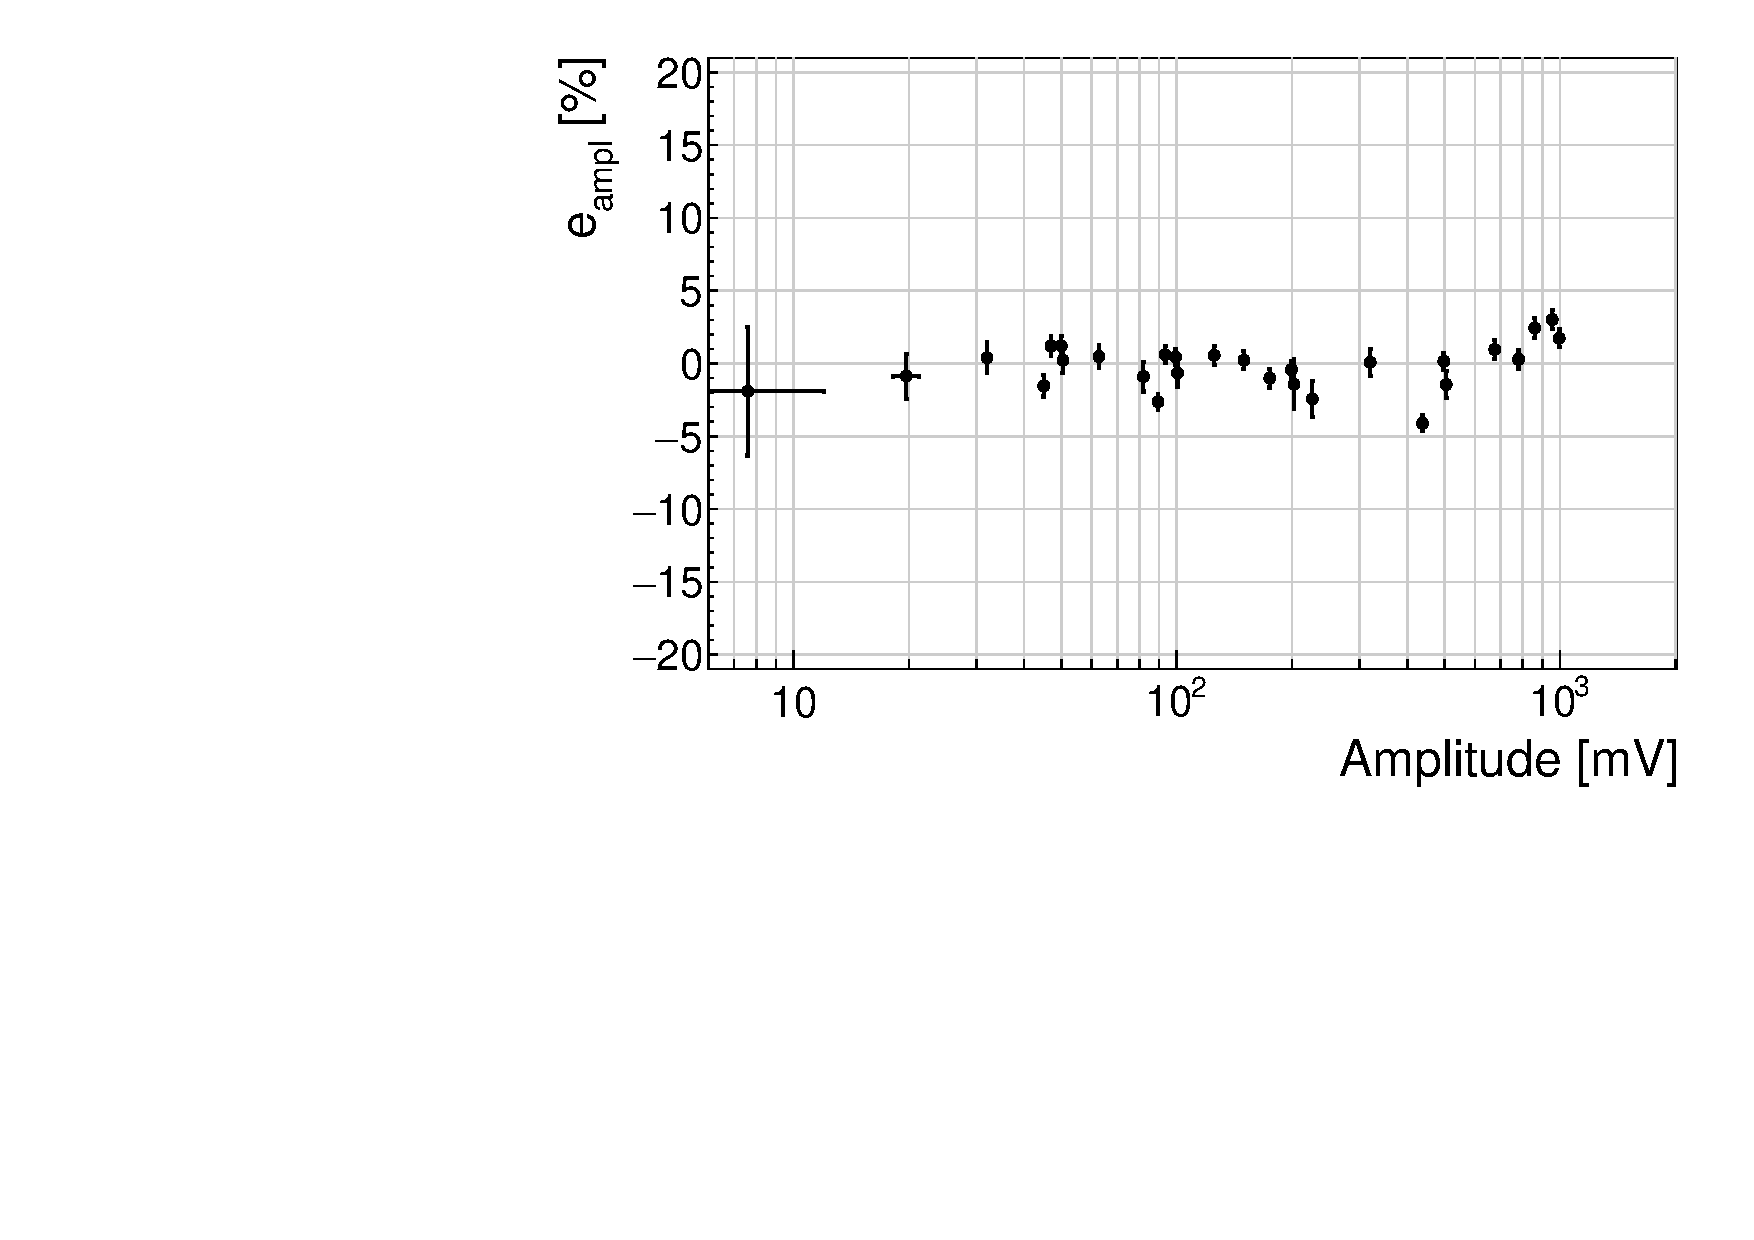
\includegraphics[width=0.45\textwidth]{../scripts/05_current_monitoring/PulseGenTests/plots/ratioAmpl1} \label{fig:ratioAmpl1}} &
\subfloat[Amplitude stability]{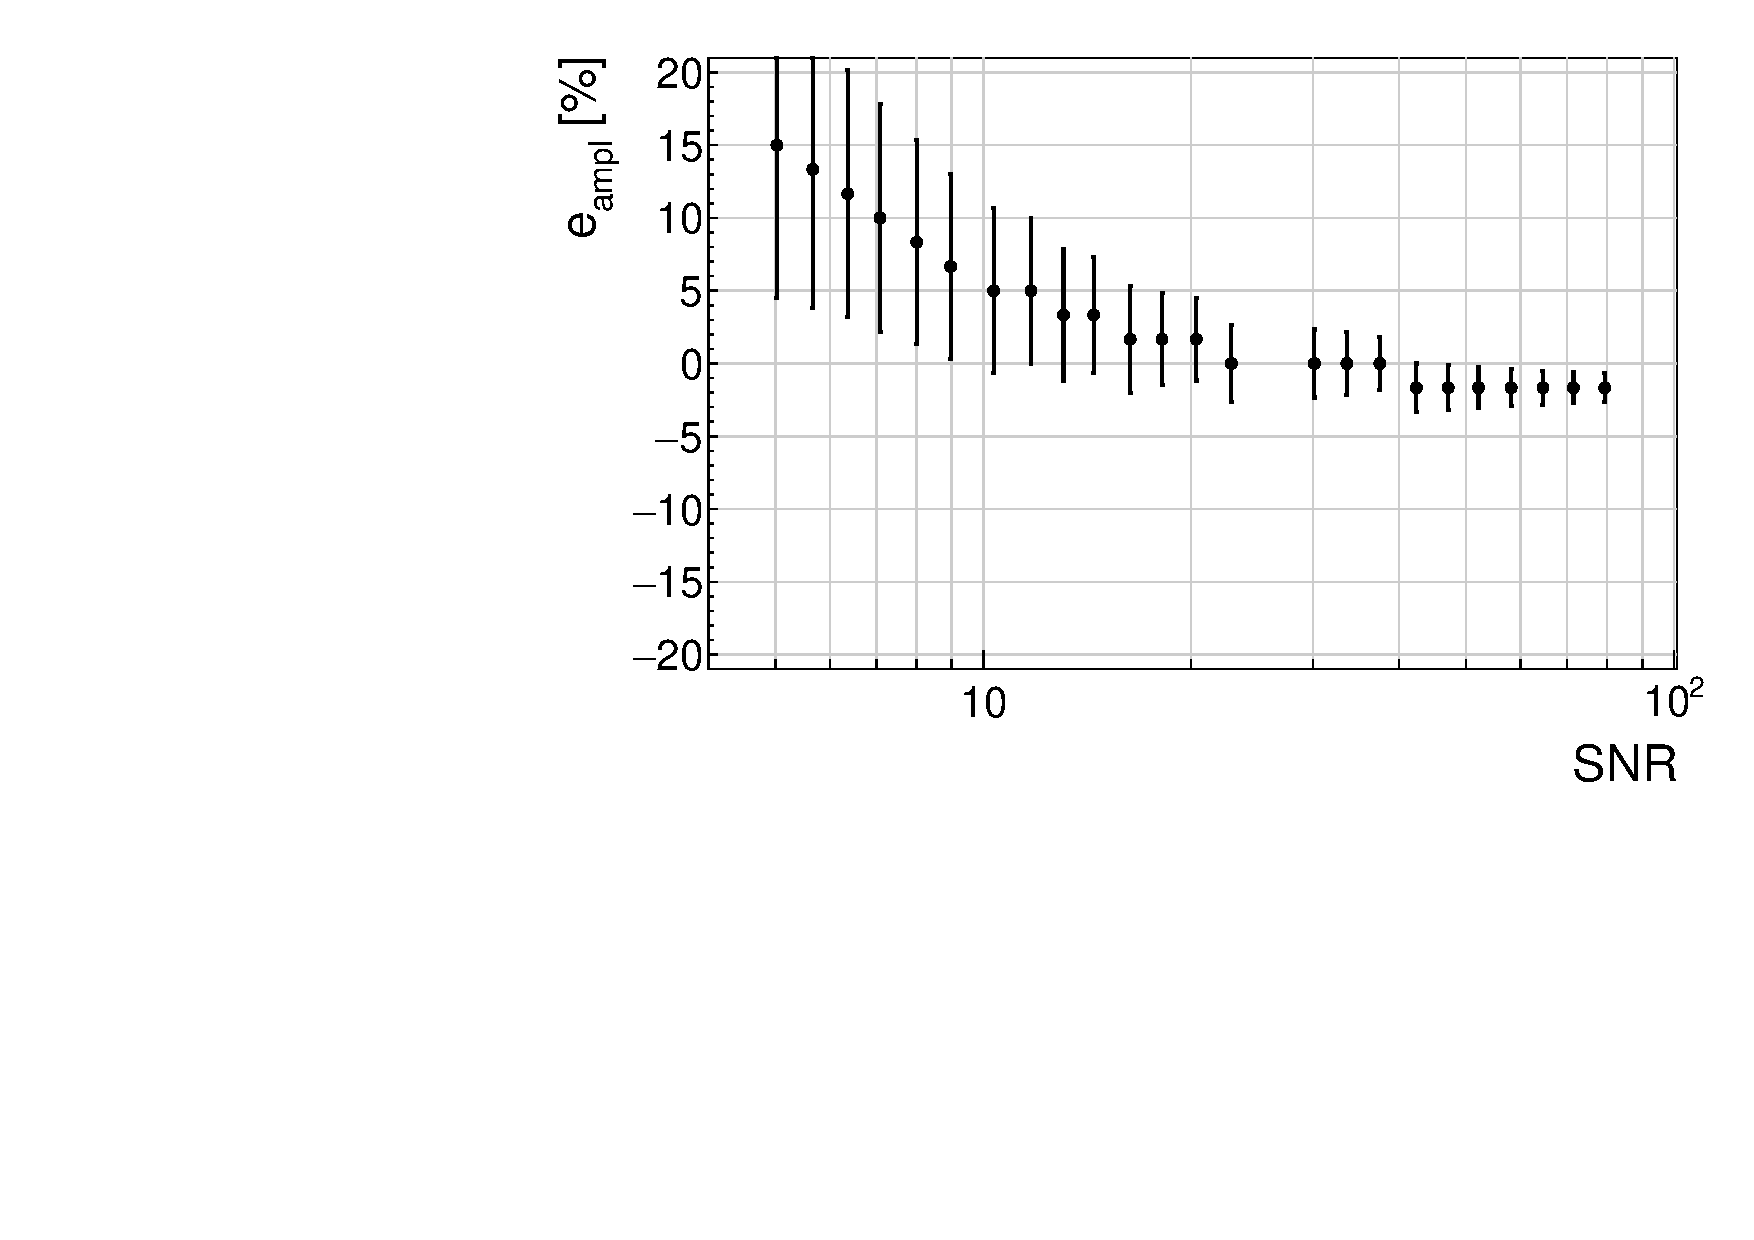
\includegraphics[width=0.45\textwidth]{../scripts/05_current_monitoring/PulseGenTests/plots/snrAmpl1} \label{fig:snrAmpl1}} \\

\subfloat[Linearity across the width range]{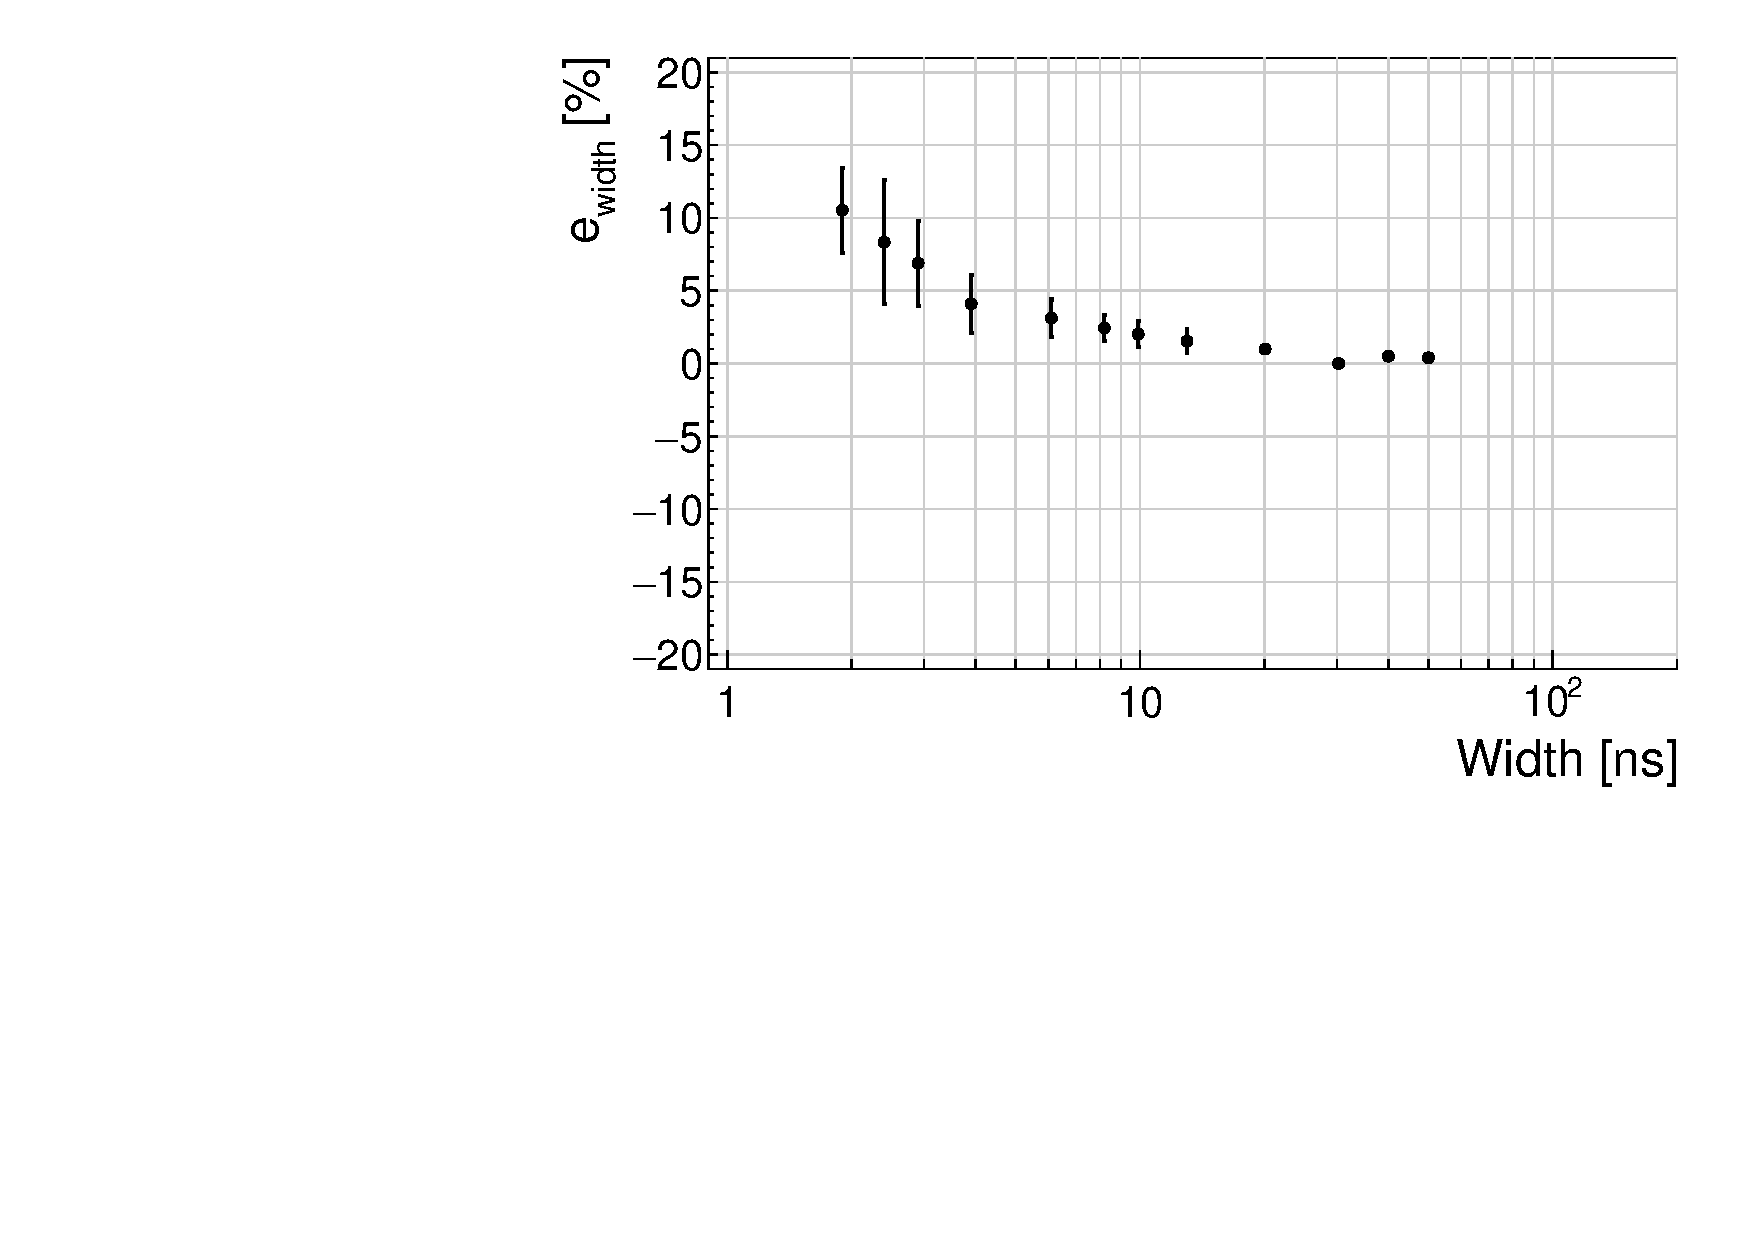
\includegraphics[width=0.45\textwidth]{../scripts/05_current_monitoring/PulseGenTests/plots/ratioWidth1}  \label{fig:ratioWidth1}} &
\subfloat[Width stability]{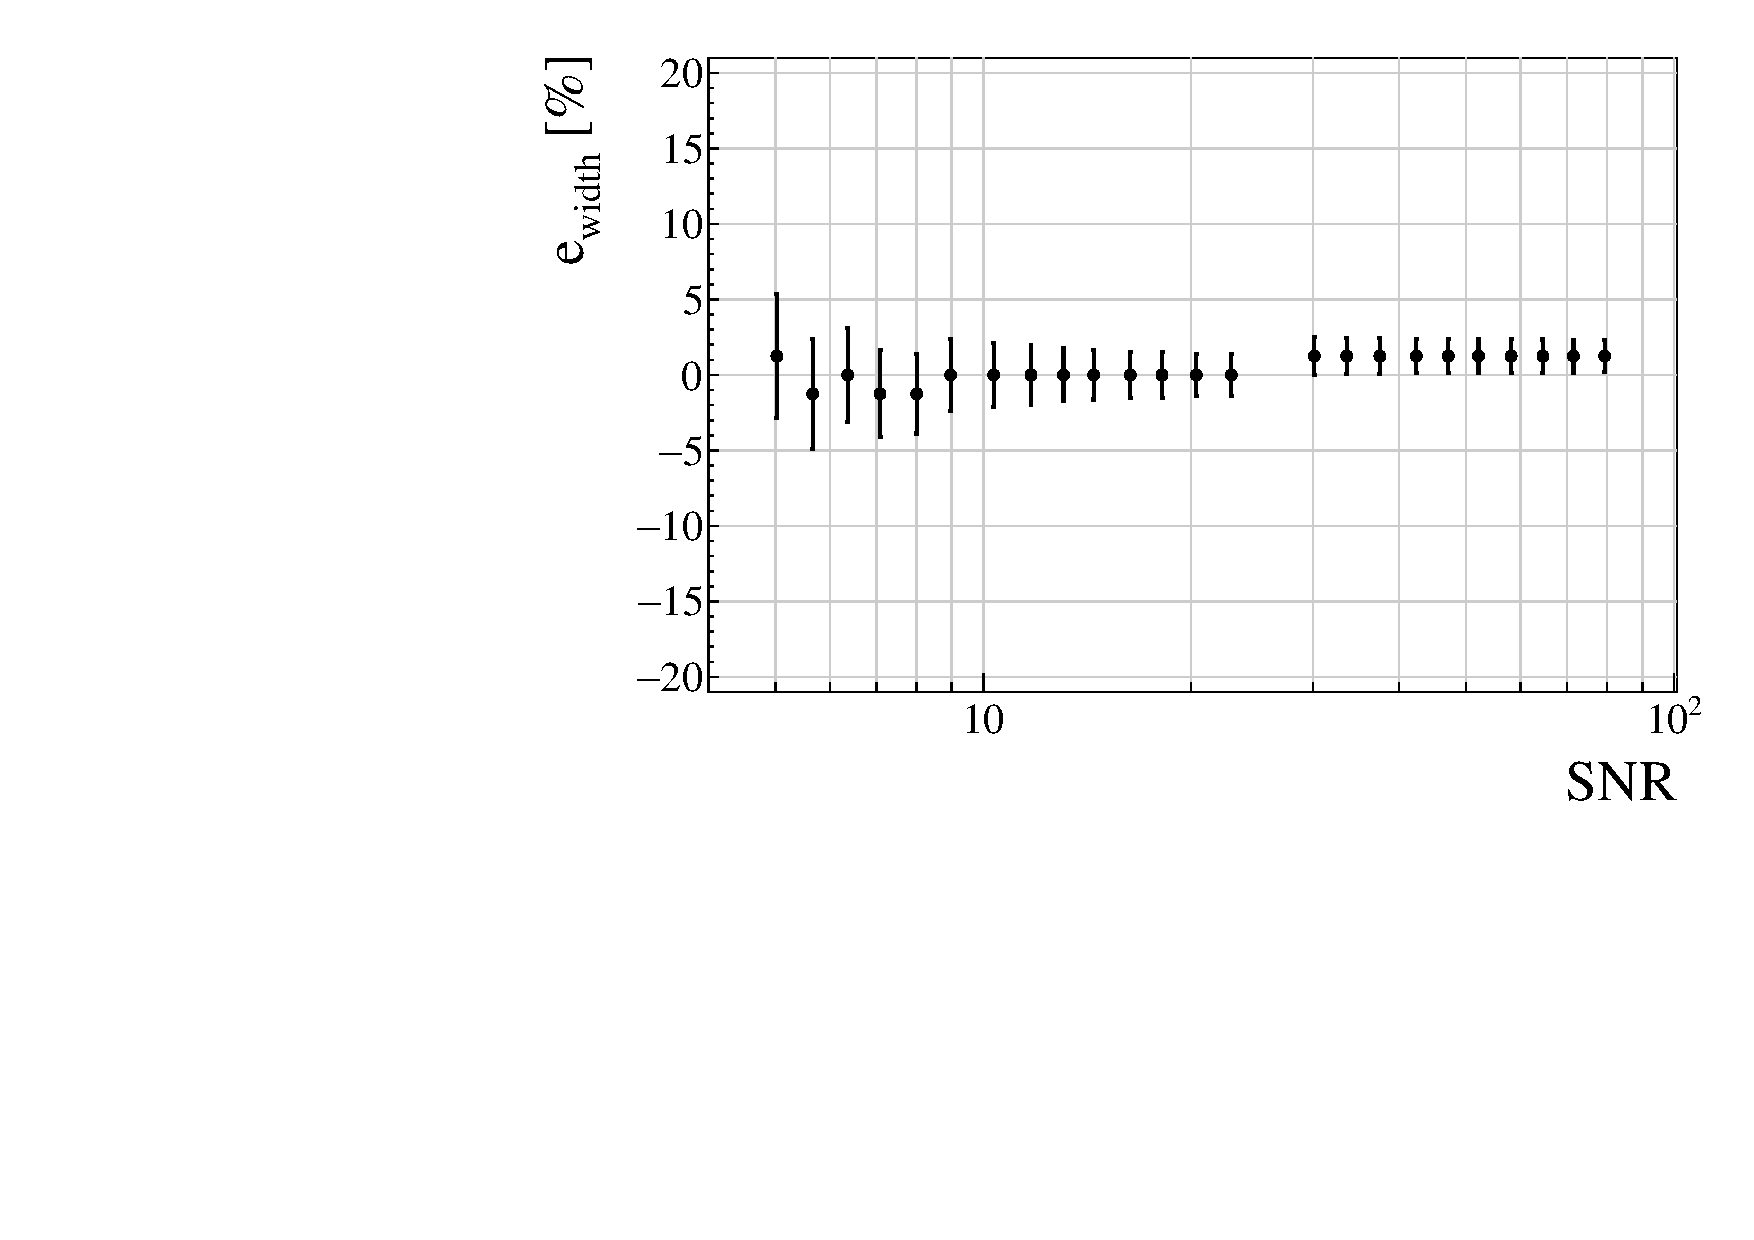
\includegraphics[width=0.45\textwidth]{../scripts/05_current_monitoring/PulseGenTests/plots/snrWidth1}  \label{fig:snrWidth1}} \\
 &
%\subfloat[Linearity across the area range]{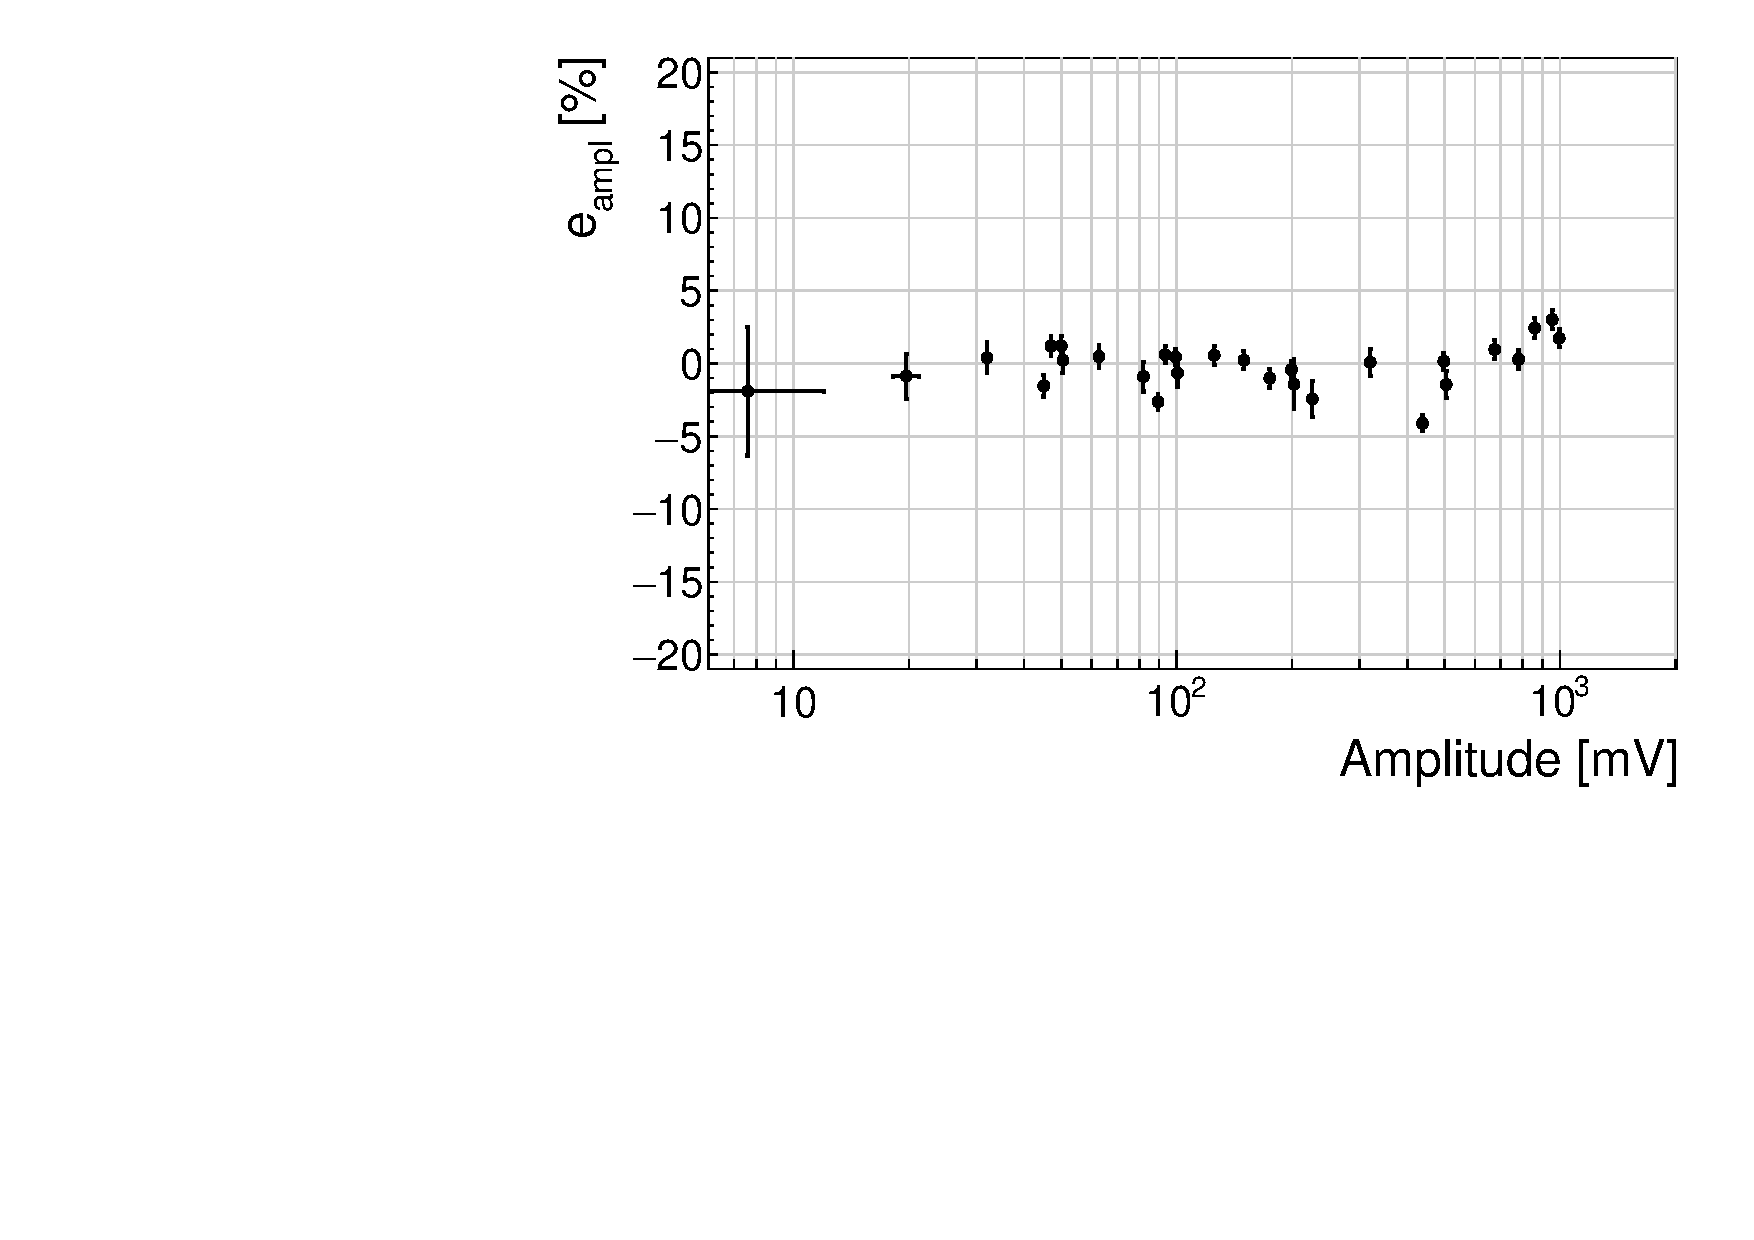
\includegraphics[width=0.45\textwidth]{../scripts/05_current_monitoring/PulseGenTests/plots/ratioAmpl1}  \label{fig:ratioArea1}} \\
\subfloat[Area stability]{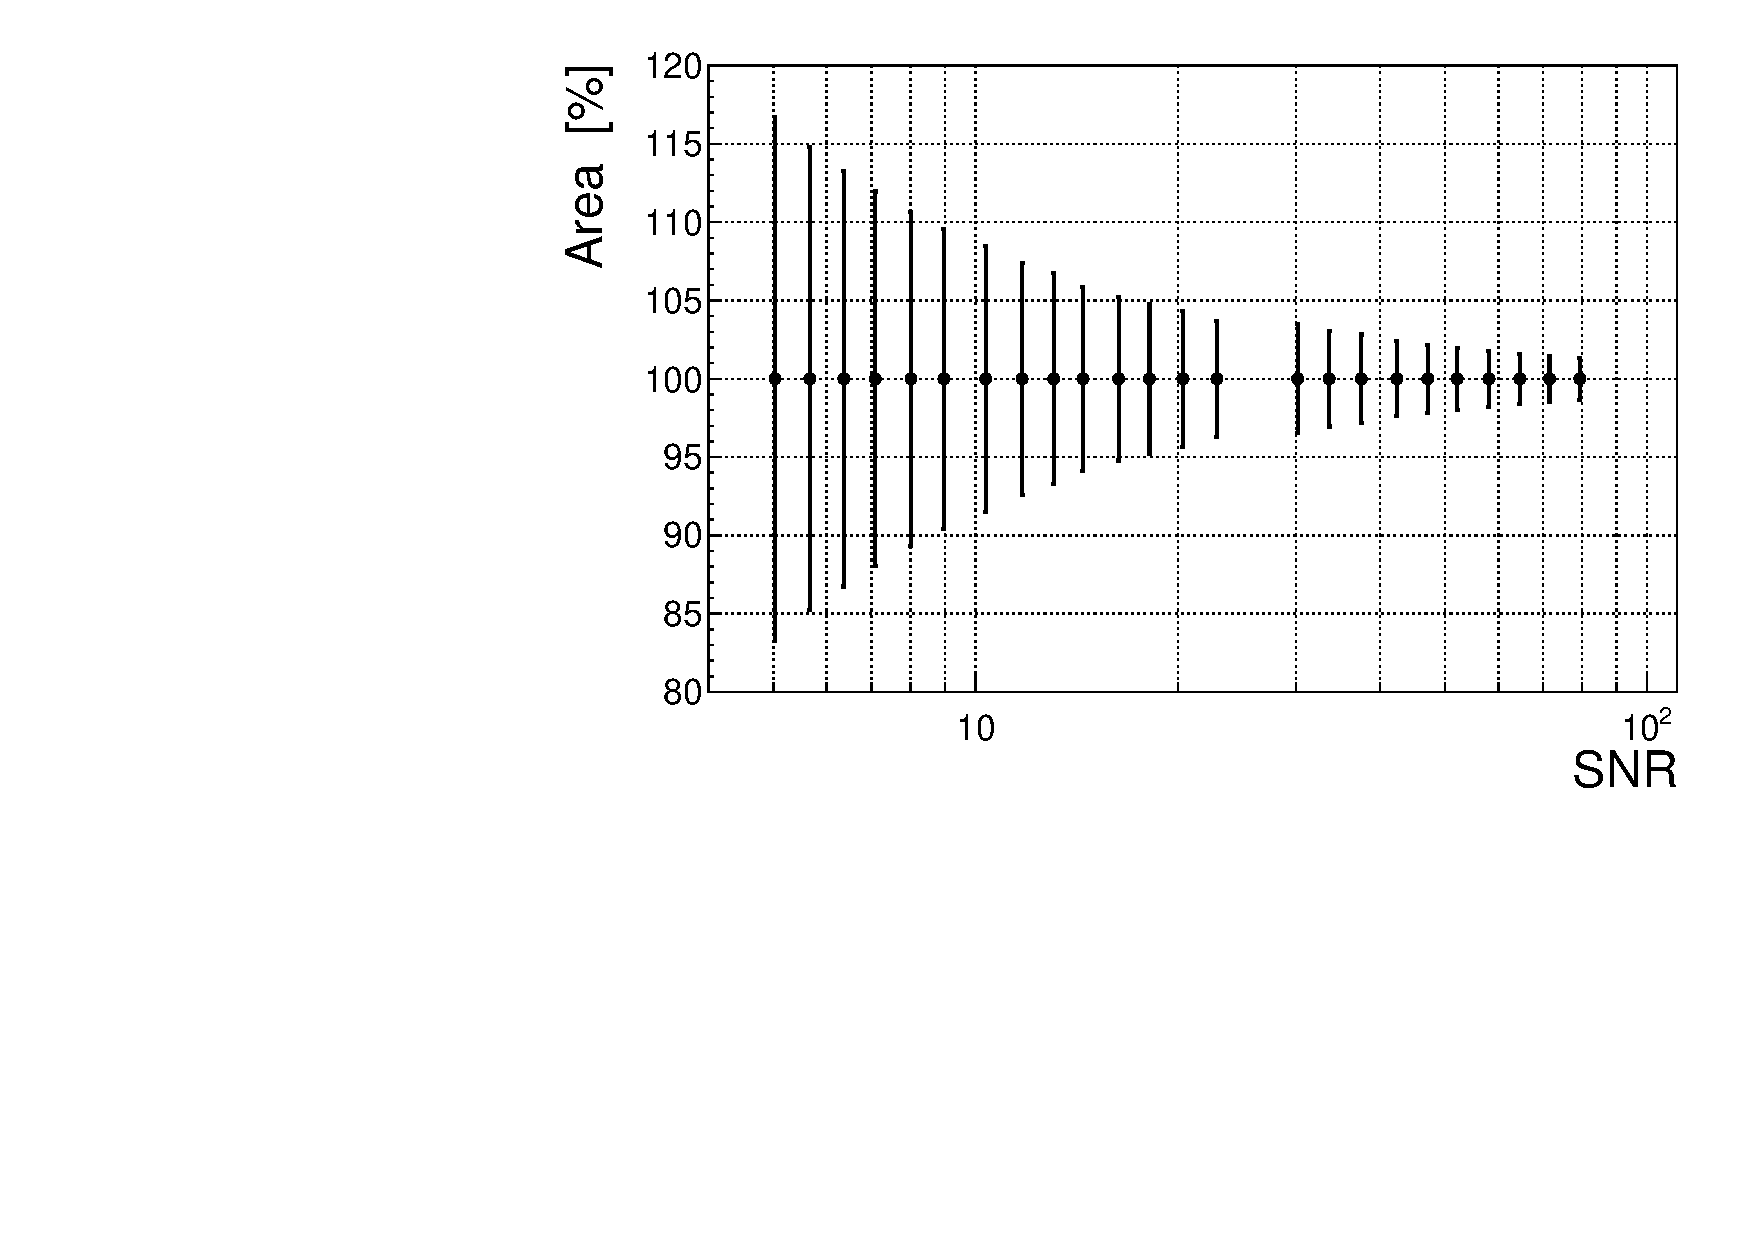
\includegraphics[width=0.45\textwidth]{../scripts/05_current_monitoring/PulseGenTests/plots/snrArea1}  \label{fig:snrArea1}}
\end{tabular}
\caption{These diagrams show the linearity of the measurements and their stability with respect to analog noise.}
\label{fig:ratiosnr}
\end{figure}



\subsection{Comparison between the charge- and current-sensitive spectroscopy}
The calibration was done using a \textsuperscript{148}Gd\textsuperscript{239}Pu\textsuperscript{241}Am\textsuperscript{244}Cm source which emits $\upalpha$ particles with four different energies. The PSA in combination with the current amplifier was compared against the 8-bit spectroscopic application in combination with the charge amplifier and a commercial 14-bit spectroscopic readout.

\begin{figure}[!t]
\centering
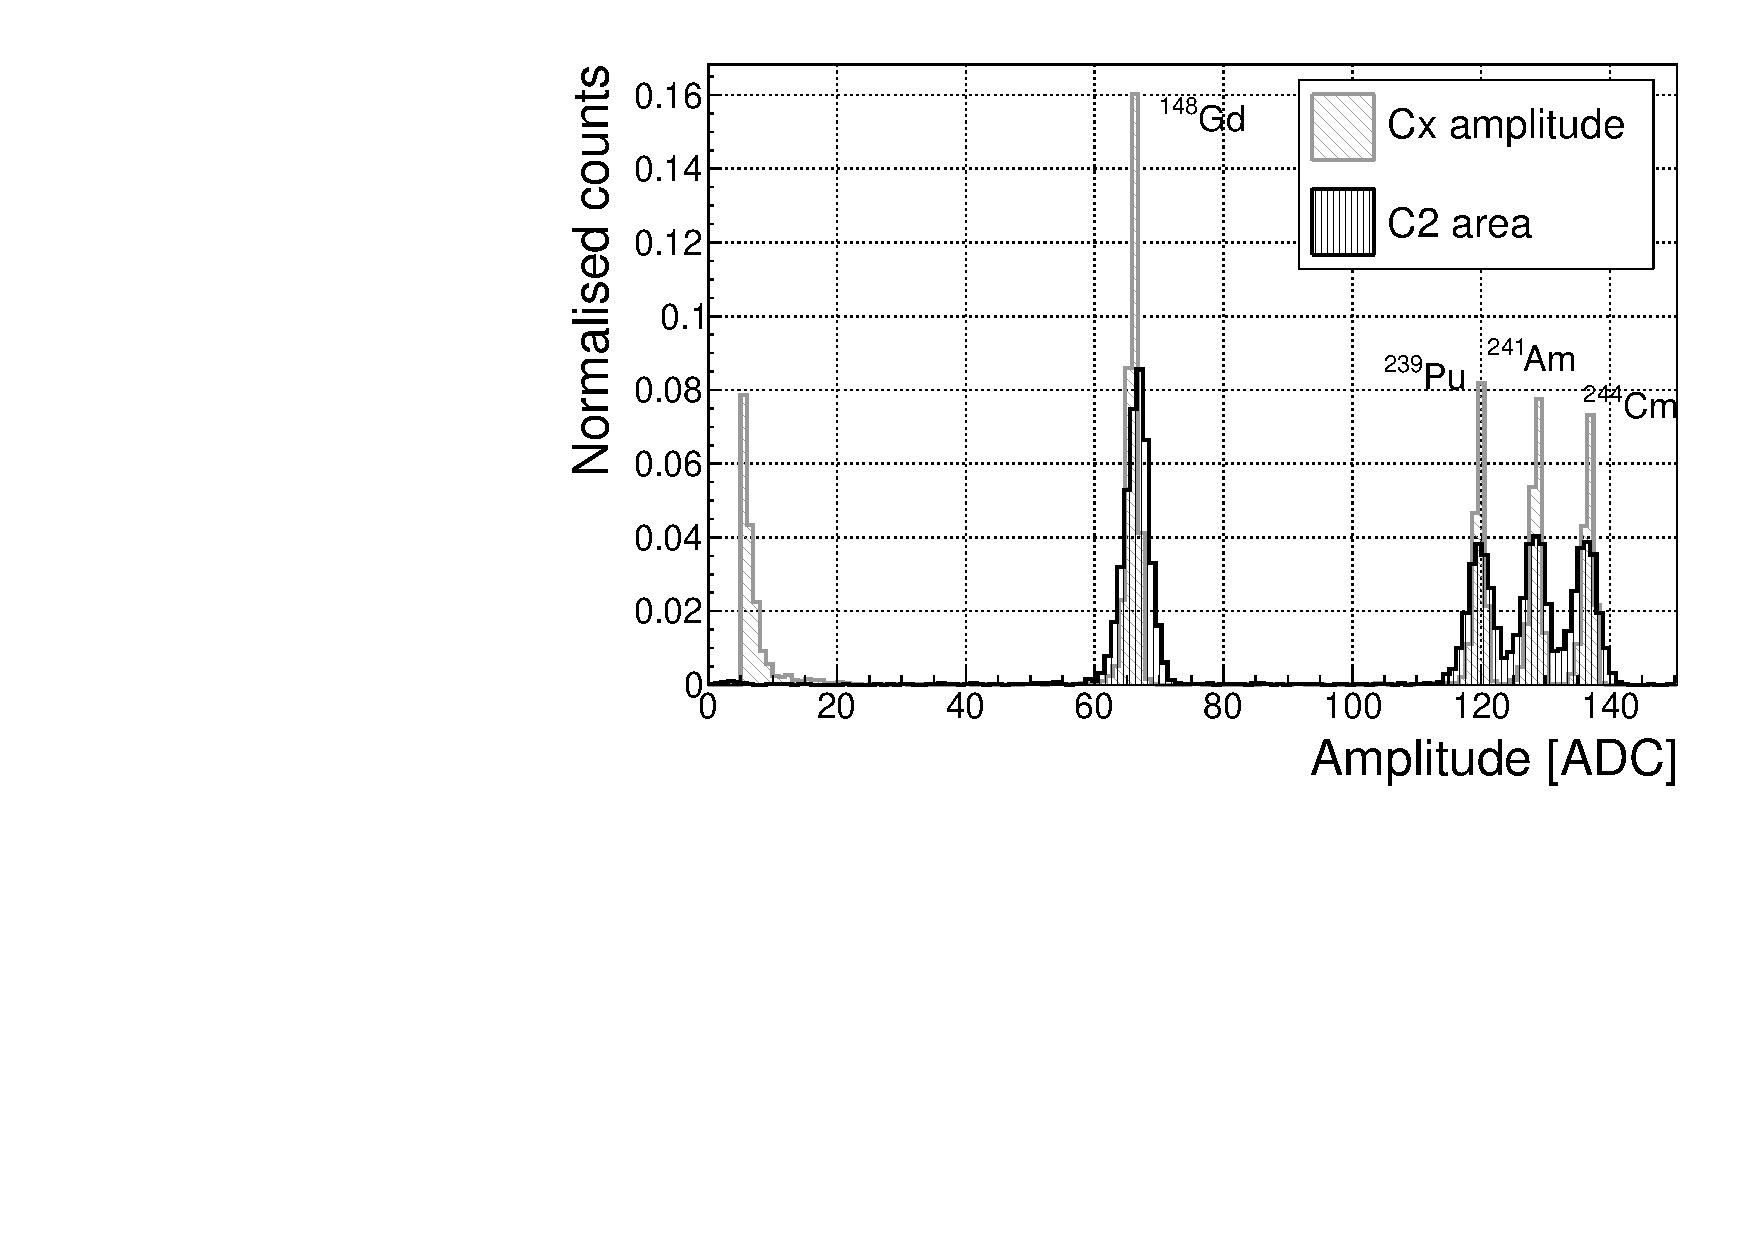
\includegraphics[width=0.8\textwidth]{../scripts/05_current_monitoring/plot4alpha/plots/4alphaCompare}
\caption{Spectrum of a \textsuperscript{148}Gd\textsuperscript{239}Pu\textsuperscript{241}Am\textsuperscript{244}Cm source using a Cx and a C2 amplifier}
\label{fig:c2cx4alpha}
\end{figure}
The $^{241}$Am peak measured by the Cx amplifier has an RMS of 0.8~ADC, which corresponds to a 32~keV energy resolution. For comparison, the C2 amplifier measures this peak with an RMS of 1.9~ADC, which corresponds to a 75~keV energy resolution. Therefore the energy spectrum measured by the current amplifier has a lower energy resolution.


%\subsection{Pulse identification test}
%The device was tested using two radioactive sources at the same time. The $^{241}Am$ source of 5.12~MeV $\upalpha$ particles was placed on one side of the diamond. The $^{60}$Co source of photons with the energy of 1.3~MeV was placed on the other side. The diamond was put in the vacuum chamber to reduce the energy loss of $\upalpha$ particles in the air. The chamber also provided good shielding, reducing the noise pick-up significantly. 
%alpha and cobalt







% ---------------------------------------------------------------------------------------------------------------
\clearpage
\section{Source calibration}
\label{sec:sourcecalib}
% ---------------------------------------------------------------------------------------------------------------
The operation of the pulse shape analysis has been tested using several radioactive sources. In particular, an $\upalpha$, a $\upbeta$ and a $\upgamma$ source have been used. Each source has been placed on top of the diamond detector and left for a predefined time depending on its activity. Table~\ref{tab:semicompare} shows the sources used, the time of exposure and their rate during this time. The data for the $\upalpha$ source have been taken for both polarities. In addition, a long run with an $\upalpha$ source with a sheet of paper in between the source and the diamond has been taken. The paper stops the $\upalpha$ particles but lets through the photons, which helps to estimate the background photon radiation of the source.

\begin{footnotesize}
\begin{center}
\begin{tabular}{l c c c c c c c}
\hline
Run & Source & Radiation & Energy [MeV] & Time [h]  & Triggers & Rate [s$^{-1}$]  & Bias [V]   \\
\hline
1&$^{241}$Am*  & $\upalpha$ & 5.5 & 60 & 958 & 4.4e-3  & 500 \\
2&$^{241}$Am  & $\upalpha$ & 5.5 & 17 & 10558 & 0.17  & 500 \\
3&$^{241}$Am  & $\upalpha$ & 5.5 & 18 & 11454 & 0.18 & -500 \\
4&$^{90}$Sr  & $\upbeta$ & 2.3 & 0.42 & 1.07e6 & 1000 & 500 \\
5&$^{60}$Co  & $\upgamma$ & 1.3 & 0.28 & 1.34e6 & 3300 & 500 \\
6&$^{239}$Pu~Be  & $n$ & 1--10 & 2.5 & 1.5e6 & 230 & 500 \\ 
\hline
\end{tabular}
\captionof{table}{Measurements carried out at Atominstitut}
\label{tab:semicompare}
\end{center}
\end{footnotesize}

The pulses acquired during the data taking are shown in persistence plots in figures~\ref{fig:accpulses}. Figure~\ref{fig:am1} showing the $^{241}$Am source background reveals that the diamond detector had been contaminated, probably with chipped-off grains of the unsealed source. This stems from the fact that $\upalpha$ pulses are recorded despite having a sheet of paper, which stops all the particles emitted by the source. 
However, the number of $\upalpha$ hits due to contamination is negligible - an estimated 1~h$^{-1}$. Another point worth noting is the falling slope of the rectangular pulse in figure~\ref{fig:am3}. This stems from the space charge that had built up during the neutron irradiation and is discussed in section~\ref{sec:spacecharge}. Finally, figure~\ref{fig:pu1} shows that the neutron source causes the widest variety of pulse shapes - triangular and rectangular as well as those in between. Pulse shapes caused by neutrons are described in detail in~\cite{PAVEL:00003, CHRISSI:00005}.

% ATI source measurements
\clearpage
\begin{figure}[!t]
%\centering
\begin{tabular}{rrr}
\subfloat[$^{241}$Am background]{\includegraphics[width=0.44\textwidth]{../../../CIVIDEC/dataRead/data/plots/reportATI/27-pulse-background-1} \label{fig:am1}} &
\subfloat[$^{241}$Am, e$^{-}$ collection]{\includegraphics[width=0.44\textwidth]{../../../CIVIDEC/dataRead/data/plots/reportATI/10-pulse-alpha-e-0}  \label{fig:am2}} \\
\subfloat[$^{241}$Am, h$^+$ collection]{\includegraphics[width=0.44\textwidth]{../../../CIVIDEC/dataRead/data/plots/reportATI/18-pulse-alpha-h-0}  \label{fig:am3}} &
\subfloat[$^{90}$Sr]{\includegraphics[width=0.44\textwidth]{../../../CIVIDEC/dataRead/data/plots/reportATI/13-pulse-beta-0} \label{fig:sr1}} \\
\subfloat[$^{60}$Co]{\includegraphics[width=0.44\textwidth]{../../../CIVIDEC/dataRead/data/plots/reportATI/12-pulse-gamma-0}  \label{fig:co1}} &
\subfloat[$^{239}$Pu~Be]{\includegraphics[width=0.44\textwidth]{../../../CIVIDEC/dataRead/data/plots/reportATI/15-pulse-neutron-0}  \label{fig:pu1}} 
\end{tabular}
\caption{Accumulated pulses for all runs}
\label{fig:accpulses}
\end{figure}
\clearpage

\subsection{Source measurements -- scatter plots}
An online pulse shape analysis has been run on all the above mentioned data sets. The parameters of the pulses are plotted in 2D histograms - in form of scatter plots. The aim is to find a way to distinguish between the various types of radiation in order to only select the spectrum of a single type of particles from a spectrum of a mixed source. The energy spectrum is directly proportional to the measured area of the current pulses, therefore all the parameters are plotted against the pulse area. The parameters used are: 
\begin{itemize}
\item FWHM
\item Base width
\item Amplitude
\item Amplitude $\times$ Base width
\item Base width -- FWHM
\item Falling slope
\end{itemize}
Every individual parameter can be attributed a set of qualifiers with which a certain part of the distribution can be rejected. There are two ways to apply the qualifiers. One is to set the minimum and maximum value for a specific parameter. The accepted pulses are those in between these two values. The minimum and the maximum qualifier are marked with a blue and a red line in the subsequent scatter plots. The second way is to apply a linear cut to the distribution in the scatter plot. The user can choose the slope of the line and to accept either the pulses above or below the line. The colour of the line is blue if the part above the line is accepted and red if opposite. Currently two scatter plots have this option implemented: area vs amplitude and area vs amplitude$\times$base width. The latter represents the Form Factor, which is discussed in section~\ref{subsec:algorithm}.

The sets of plots in figures~\ref{fig:scatterae}, \ref{fig:scatterah}, \ref{fig:scattersr} and \ref{fig:scatterco} show the above listed parameters plotted against the pulse area for $^{241}$Am background, electrons and holes, $^{90}Sr$ and $^{64}$Co source, respectively. Any distinguishable difference between the plots of two sources would suggest that that particular parameter can be used to distinguish one type radiation from the other. For the most part the photons are considered the rejected pulses (greyscale colour palette) whereas $\upalpha$ particles or neutrons are accepted (yellow colour palette). In special cases only a certain types of neutron interactions are accepted (see section~\ref{sec:nm}).

 

% alpha: gamma background. alphas of all energies (air).
% gamma, beta - overlapping
%\clearpage
%\begin{figure}[!t]
%\centering
%\includegraphics[width=0.99\textwidth]{../../../CIVIDEC/dataRead/data/plots/reportATI/29-scatter-0}
%\caption{Background measurements}
%\label{fig:scatterbm}
%\end{figure}
\subsubsection{$^{241}$Am source}
The source emits $\upalpha$ particles at $\sim$5.5~MeV and photons with a range of energies. Due to the losses in the air and the electrode the measured $\upalpha$ energy varies -- between $\sim$5~MeV down to 1~MeV. 

Figures~\ref{fig:scatterae} and~\ref{fig:scatterah} show the pulse area distribution with respect to the aforementioned parameters, for electrons and holes respectively. 
Focusing on the top left plot in figure~\ref{fig:scatterae}, a distinctive horizontal stripe appears at a width of 9~ns, ranging from 100 up to 630~pVs. This is the aforementioned spread of $\upalpha$ energies. The shape of the pulse from this type of radiation retains the width even at smaller energies. Only its amplitude is decreased. This is because the free charge carriers in the diamond are traveling with the same speed in all cases, inducing rectangular pulses of the same widths. 

The other cluster in the [area, FWHM] phase space comes from the background photons. The two clusters are far apart from one another with no overlap. It is therefore straightforward to define a cut in the FWHM to distinguish between the $\upalpha$ and $\upgamma$ entries. This is done by means of the minimum and maximum FWHM constant qualifier, which marked red and blue in the [area, FWHM] subfigure.

The [area, amplitude] subfigure also reveals two distinguishable clusters, which can be segregated using a linear qualifier. The angle of the $\upalpha$ stripes in the [area, amplitude] subplots is significantly smaller than that of the photon stripe. The separation is much less pronounced in the other subfigures. 

There is a third barely distinguishable island visible in the top two plots, both area and width values close to zero. This island is formed by noise, which triggered the analysis.

The situation is similar when inverting the bias voltage and collecting holes (see figure~\ref{fig:scatterah}). Here, however, the two clusters are much closer together even in the [area, FWHM] subfigure. This makes it more difficult to define a clear border between the two. The other five qualifiers are in this case less important than the FWHM. Nevertheless, it can be deduced from the plots that the difference BW-FWHM must be below 4~ns.

The slope is dependent of the amplitude, which can be seen in the bottom right plot, making it an unreliable qualifier in the lower area range. The amplitude, scaling with area, makes a distinguishable straight line in the middle left subfigure. 

The amplitude increase with area in the [area, amplitude] subfigure is similar for photons and $\upalpha$ particles. Therefore a linear qualifier can not be used to distinguish $\upalpha$ radiation from $\upgamma$ radiation when measuring holes.


%\clearpage
\begin{figure}[!t]
\centering
\includegraphics[width=0.99\textwidth]{../../../CIVIDEC/dataRead/data/plots/reportATI/10-scatter-0_add}
\caption{$^{241}$Am, e$^{-}$ collection. Qualifier: FWHM. Optional qualifiers: Amplitude, Form Factor.}
\label{fig:scatterae}
\end{figure}

%\clearpage
\begin{figure}[!t]
\centering
\includegraphics[width=0.99\textwidth]{../../../CIVIDEC/dataRead/data/plots/reportATI/18-scatter-0}
\caption{$^{241}$Am, h$^{+}$ collection. Qualifier: FWHM.}
\label{fig:scatterah}
\end{figure}

Figures~\ref{fig:1dearea} and~\ref{fig:1dharea} show a one-dimensional area distribution of the acquired data for electron and hole collection. The blue histogram represents all collected data whereas the red one marks the data whereby the pulse parameters are within the qualifiers. In both figures the $\upalpha$ peak at 600~pVs is clearly visible, followed by a $\upgamma$ quasi-Landau distribution with an MPV of $\sim$70~pVs and a noise peak at the very left of the area distribution. These two contributions have been rejected by the FWHM qualifier.

\begin{figure}[!t]
\centering
\begin{tabular}{cc}
\subfloat[$^{241}$Am, e$^{-}$ collection]{\includegraphics[width=0.7\textwidth]{../../../CIVIDEC/dataRead/data/plots/reportATI/10-area-0} \label{fig:1dearea}} \\
\subfloat[$^{241}$Am, h$^+$ collection]{\includegraphics[width=0.7\textwidth]{../../../CIVIDEC/dataRead/data/plots/reportATI/18-area-0}  \label{fig:1dharea}}
\end{tabular}
\caption{$^{241}$Am area histograms for electron and hole collection.}
\label{fig:1dalphaarea}
\end{figure}

\clearpage
\subsubsection{$^{90}$Sr and $^{60}$Co source}
The phase space of the $^{90}$Sr source overlaps entirely with that of the $^{60}$Co source (see figures~\ref{fig:scattersr} and \ref{fig:scatterco}). This renders it virtually impossible to distinguish between photons and electrons (MIPs). Comparing the [area, FWHM] phase space of the photons and alphas and the high reach of the former, the electron collection of the alphas would need to be used to distinguish between the two types of particles. 

The one-dimensional histograms in figure~\ref{fig:1dcosrarea} show a quasi-Landau distribution with the MPV at $\sim$70~pVs, which is in agreement with the background $\upgamma$ radiation emitted by the $^{241}Am$~source (see figure~\ref{fig:1dalphaarea} in the previous subsection). This is however not a pure Landau distribution. Relative to the 600~pVs $\upalpha$ peak, the expected MPV of MIPs would be $\sim$30~pVs, which is not the case in these distributions. This is because the PSA device is a self-triggering system, which cuts the lower energetic particles with the trigger threshold. The resulting distribution is therefore only the top portion of the real Landau distribution. Unfortunately this is the limitation of the device, governed by the analog noise of the current pre-amplifier.

\begin{figure}[]
\centering
\includegraphics[width=0.99\textwidth]{../../../CIVIDEC/dataRead/data/plots/reportATI/13-scatter-0}
\caption{$^{90}$Sr scatter plots}
\label{fig:scattersr}
\end{figure}


\begin{figure}[]
\centering
\includegraphics[width=0.99\textwidth]{../../../CIVIDEC/dataRead/data/plots/reportATI/12-scatter-0}
\caption{$^{60}$Co scatter plots}
\label{fig:scatterco}
\end{figure}

\begin{figure}[]
\centering
\begin{tabular}{cc}
\subfloat[$^{90}$Sr]{\includegraphics[width=0.7\textwidth]{../../../CIVIDEC/dataRead/data/plots/reportATI/13-area-0} \label{fig:1dsrarea}} \\
\subfloat[$^{60}$Co]{\includegraphics[width=0.7\textwidth]{../../../CIVIDEC/dataRead/data/plots/reportATI/12-area-0}  \label{fig:1coharea}}
\end{tabular}
\caption{Energy distributions for $\upgamma$ and $\upbeta$ particles.}
\label{fig:1dcosrarea}
\end{figure}

%\clearpage
%\begin{figure}[!t]
%\centering
%\includegraphics[width=0.99\textwidth]{../../../CIVIDEC/dataRead/data/plots/reportATI/15-scatter-0}
%\caption{$^{239}$Pu~Be. Qualifiers: BW-FWHM 0.2--4~ns, FWHM 3--12~ns, Form factor 1.45}
%\label{fig:scatterpu}
%\end{figure}
%
%\clearpage
%\begin{figure}[!t]
%\centering
%\includegraphics[width=0.99\textwidth]{../../../CIVIDEC/dataRead/data/plots/reportATI/15-scatter-1}
%\caption{$^{239}$Pu~Be. Qualifiers: BW-FWHM 0.2--4~ns, FWHM 3--12~ns, Slope 25--104~mV/ns}
%\label{fig:scatterpu2}
%\end{figure}



% ---------------------------------------------------------------------------------------------------------------
%\subsection{Space charge build-up}
%\label{sec:spacecharge}
%Space charge built up during the neutron irradiation ($\sim10^{10}~$n), which reflected on the pulse shapes. Instead of a flat top, they developed a slope. This was of opposite signs for the two polarities, as can be seen in figures~\ref{fig:sc1} and~\ref{fig:sc2}. The figures contain a set of 64 superimposed pulses taken at $\pm$500~V bias. The shape persisted until the space charge was neutralised by means of a $\upbeta$ source irradiation at a 0~V bias. Figure~\ref{fig:sm} shows the decreasing of the slope coefficient as a function of received $\upbeta$ dose.
%
%
%\begin{figure}[!t]
%\centering
%\begin{tabular}{rrr}
%\subfloat[$^{241}$Am, e$^{-}$ collection]{\includegraphics[width=0.44\textwidth]{../../../CIVIDEC/dataRead/data/plots/reportATI/16-pulse-alpha-sc-1} \label{fig:sc1}} &
%\subfloat[$^{241}$Am, h$^+$ collection]{\includegraphics[width=0.44\textwidth]{../../../CIVIDEC/dataRead/data/plots/reportATI/17-pulse-alpha-sc-1}  \label{fig:sc2}} \\
%\end{tabular}
%\caption{Built up space charge causes a slope which has the opposite slope for electrons and holes}
%\label{fig:sc}
%\end{figure}
%
%\begin{figure}[!t]
%\centering
%\includegraphics[width=0.8\textwidth]{../../../CIVIDEC/dataRead/data/plots/spaceChargeStudy}
%\caption{Using $\upbeta$ radiation to reduce space charge in diamond}
%\label{fig:sm}
%\end{figure}


























% ---------------------------------------------------------------------------------------------------------------
\clearpage
%\section{Neutron reactor measurements}
\section{Applications in neutron instrumentation}
\label{sec:nm}
% ---------------------------------------------------------------------------------------------------------------

The real-time pulse shape analysis procedure can be applied to more complex systems. This section includes three applications where the PSA has been applied.

Semiconductor-based neutron detectors provide a compact technology for neutron detection. However, the cross section of a neutron with the diamond bulk is very low, since it only interacts with the core of the atom. Diamond is mainly used to detect charged particles and photons. 

Research neutron reactors radiate a mix of particles, apart from neutrons also photons. The photons are considered a background radiation, concealing the neutron spectrum. When measured with diamond, the signal from neutrons is difficult to distinguish from the photon spectrum. In addition, low energy neutrons do not cause nuclear reactions in the bulk. All in all, the neutron measurements in a reactor present a challenge with diamond. However, by means of the PSA, the neutron signal can be discriminated from the photon background to some extent. The following two cases show how measurements of fast (n$^+$) and thermal (n$^-$) neutrons have been carried out by making use of the PSA.

Note the changing scale on the X axis in the figures.


%----------------------------------------------------------
\subsection{Thermal neutron flux monitoring}
Research neutron reactors like TRIGA MARK II~\cite{TRIGA:00001} at Atominstitut~\cite{ATOM:00001} in Vienna are capable of emitting neutrons at a wide range of energies. The neutron flux is proportional to the current power of the reactor. It is therefore instrumental to monitor the neutron flux to make sure that the reactor operation is within the specified limits. However, the byproduct of the radioactive decays in the core is $\upgamma$ radiation, which has an energy range that overlaps with that of neutrons, making it difficult to measure the neutron flux. This is where PSA and diamond detectors come into play. This section describes the application of thermal neutron flux monitoring by means of the PSA.

Thermal neutrons do not interact with the diamond bulk due to their low kinetic energy (of the order of 0.012~eV). Hence a converter foil has to be added to produce second order effects. Incoming neutrons interact with the foil, producing a set of secondary particles. These can then be detected upon hitting the detector bulk. Common neutron interactions that are used in thermal neutron detection are \textsuperscript{10}B(n,$\alpha$)\textsuperscript{7}Li reaction and \textsuperscript{6}Li(n,$\alpha$)\textsuperscript{3}H reaction ($\alpha$ stands for $^4_2$He, see equation~\ref{eq:reaction}). The focus in this section is on the latter. With a foil installed, there are several possibilities for neutrons to interact with the detector system. Each of these interactions ionises the diamond bulk in its own way, resulting in a specific shape of the current pulse. A neutron can: 1) interact with the foil, producing an $\upalpha$ and a \textsuperscript{3}H, 2) interact with a carbon atom in the lattice, producing an $\upalpha$ and a $\upgamma$ or even three $\upalpha$. The thermal neutrons do not have enough kinetic energy to interact with the lattice, therefore the focus will be on case (1), the equation for this reaction is the following:
\begin{equation}
\label{eq:reaction}
   ^6_3Li   +   ^1_0n \;\rightarrow\; ^3_1H_{(2.73 MeV)} + \alpha_{(2.05 MeV)}
\end{equation}
The particles in the first case are produced outside the diamond and get stopped immediately upon hitting the sensor. The resulting pulses for both particles have a rectangular shape of the same width, because the carriers drift with the same speed in both cases. The difference is in the number of free carriers produced - the tritium creates more (proportional to the deposited energy), which in turn induces a higher pulse.

TRIGA MARK II neutron reactor emits large amounts of $\upgamma$ radiation in the energy range up to 3~MeV. This already affects the measurements of $\upalpha$ particles, the energy of which peaks at 2.05 MeV in the case of \textsuperscript{6}Li converter foil. However, $\upgamma$ background radiation can be suppressed by discriminating current pulses of photons from those induced by $\upalpha$ particles. This idea has already been implemented in offline analysis in~\cite{PAVEL:00000,PAVEL:00002}. The results show that the background photons can be subtracted successfully. In order to make sure that every single incident thermal neutron has been accounted for, the algorithm has been ported to FPGA where it detects and analyses particles in real time. 

\subsubsection{Measurements}
ROSY readout device with the implemented Pulse Shape Analysis was put to a test at Atominstitut in Vienna. Their TRIGA neutron reactor is capable of delivering thermal neutrons with the energy 0.012~eV at a rate of 10$^3$~n~cm$^{-2}$ $s^{-1}$, with a considerable $\upgamma$ background. 

First, the device was calibrated using an unsealed monochromatic $^{241}Am$ source with the emitted particle energy $E_\alpha=5.12MeV$ (taking into account the losses in the air). Then the diamond detector was exposed to the beam. Secondary reaction products ($\alpha$ and \textsuperscript{3}H particles), created by neutrons hitting the converter foil, were detected by the diamond sensor, together with a significant photon background. Then the pulse identification algorithm was applied to discriminate between the reaction products and the photons.

The main parts of the detector are an sCVD diamond sensor sized $4.7\times4.7$~cm$^2$ and a $1.8~\upmu$m thick LiF converter foil, both embedded in an RF-tight PCB. The diamond sensor is biased with a bias voltage of 1~V/$\upmu$m  and capacitively coupled to CIVIDEC's C2 40~dB wide bandwidth current preamplifier. A 5~m long BNC cable connects the preamplifier to CIVIDEC ROSY box. The detector assembly together with the preamplifier has to be placed in front of an exit hole of the reactor.

Note: this data set has been taken with an older version of the firmware, which only measured a limited number of pulse parameters.

\begin{figure}[]
\centering-
\includegraphics[width=0.99\textwidth]{../../../CIVIDEC/dataRead/data/plots/triga-08-scatter-1_add1}
\caption{Thermal neutrons, photons. Qualifier: FWHM.}
\label{fig:scattertriga1}
\end{figure}

\subsubsection{Results and discussion}
The data collected by the PSA show a high flux of photons, which covers a wide area range. The $^3$He peak is clearly visible and has almost no overlap with the photon cluster. The $\upalpha$ cluster has a much lower energy and is in the same energy range as the photons. However, if a FWHM parameter is observed, a distinction between the photons and the $\upalpha$ can be seen. By setting a qualifier to the right value, the photon background is cut away, leaving only the thermal neutron decay products in the data set (see figure~\ref{fig:scattertriga1}). The resulting one-dimensional area histogram before and after applied cuts is shown in figure~\ref{fig:areatriga0}. The blue distribution is the mixed field of background photons, tritium and $\upalpha$ particles. The latter are completely hidden in the $\upgamma$ energy distribution. After applied qualifiers the $\upalpha$ peak suddenly appears.


\begin{figure}[!t]
\centering
\includegraphics[width=0.8\textwidth]{../../../CIVIDEC/dataRead/data/plots/triga-08-area-0}
\caption{Energy spectrum after applied qualifiers reveals the tritium and $\upalpha$ peak}
\label{fig:areatriga0}
\end{figure}

\subsubsection{Conclusion}
By applying the FWHM qualifier to the acquired data from the TRIGA neutron reactor, the $\upalpha$ and tritium particles can be identified and separated from the $\upgamma$ background. The resulting cleaned data can be used to correctly count the thermal neutrons detected by the diamond sensor.












%------------------------------------------------
\subsection{Fusion power monitoring}
Many research collaborations around the world are trying to develop a functional fusion reactor, which could provide a cleaner energy source. One of them is ITER~\cite{ITER:00000}, a research fusion reactor being built in France. The idea behind it is to harvest energy from the fusion of light atoms into a heavier one. For ITER the fuel chosen is a mixture of deuterium and tritium, which fuse into a helium atom at extremely high temperatures (plasma), emitting a highly energetic neutron as a byproduct. The equation is the following:
\begin{equation}
^2_1D+^3_1T ~\rightarrow~ ^4_2He+^1_0n+17.6~MeV.
\end{equation}
The $\upalpha$ particle immediately deposits its energy within the plasma. The neutron, due to its neutral charge, continues its way out of the system where it is stopped. The stopping power is converted into energy, which heats the water into steam, which in turn spins the turbines, generating electricity.

It is possible to monitor the activity of the reactor by measuring the flux of neutrons emitted. Neutron diagnostics such as neutron cameras, neutron spectrometers and neutron flux monitors therefore provide robust measurements of fusion power. A high $\upgamma$ background makes it difficult to accurately measure the neutron flux. This is a motivation to use a diamond based detector with a real-time PSA algorithm.

The neutrons emitted are 14~MeV mono-energetic fast neutrons. The most accurate and efficient way to detect them with a diamond detector is by means of a C$_\mathrm{12}$(n,$\upalpha$) reaction with a carbon atom in the ballistic centre~\cite{PAVEL:00001}. In this region the positive and negative charge carriers created by $\upalpha$ that start drifting in the opposite directions need the same time to reach the opposite electrodes.

\subsubsection{Measurements}
The $^{239}$Pu~Be neutron source has been used to simulate the fusion reactor. It emits a mixed field of neutrons and photons with a wide range of energies. The neutrons are rarely detected with diamond -- the interactions happen mostly in the electrodes on either side of the detector. The $\upalpha$ particles created by the interactions are detected by the diamond. Depending on the side of the interaction, the created pulse is either due to hole-- or electron collection. These two interactions make the two distinct lines in the [area, FWHM] phase space (see figure~\ref{fig:scatterpu}, top left plot) at 9~ns and 6~ns. 

A very interesting interaction point is the ballistic centre~\cite{CHRISSI:00001} of the diamond. A ballistic centre is the position from which it takes the holes and the electrons the same amount of time to drift to the opposite electrodes. In this case the shortest possible pulse is created. Conversely, to conserve the collected charge and thus the pulse area, the pulse amplitude must be the highest at the ballistic centre. The entries in between are created by neutron interactions at random positions in the diamond, which produce pulses of various shapes. 
%at 4~ns is created when a neutron interacts .

\subsubsection{Results and discussion}
Coming back to the motivation, the most efficient way of counting the 14~MeV neutrons is through the measurement of the neutrons interacting in the ballistic centre~\cite{????}. To extract this type of interaction several qualifiers must be used. The first possibility is the FWHM set to 3--5~ns. However, this time the cuts on the [area, amplitude] and the [area, amplitude$\times$base value] phase space are preferred. First, a minimum constant amplitude qualifier is set to 22~mV (see figure~\ref{fig:scatterpu}, middle left plot). Then a linear amplitude qualifier is set such that only the pulses with the highest amplitude for every area value are taken. This ensures that the high pulses from the ballistic centre are chosen. Second, a maximum linear amplitude$\times$base value qualifier is set such that only the pulses bearing the closest resemblance to a rectangle are chosen (see figure~\ref{fig:scatterpu}, middle right plot). In this phase space the entries at the bottom of the distribution are bearing more resemblance to a rectangle whereas those at the top are more akin to triangles.

The resulting [area, FWHM] subfigure after applied qualifiers highlights the entries with a FWHM of 4~ns, which is the width of the pulses induced by neutrons interacting in the ballistic centre. This proves that these combined qualifiers indeed pinpoint these neutron interactions. The final one-dimensional area/energy distribution of the neutrons interacting in the ballistic centre is shown in figure~\ref{fig:scatterpuarea}. 

The result could be further improved by further constraining the identification, e.g to define the minimum FWHM constant qualifier and the minimum slope constant qualifier.


%By making use of the Form Factor set to 1.45, the three-line structure becomes more pronounced. However, a part of the cluster belonging to the 9~ns line is omitted. This part with the area ranging between 600 and 1000~pVs starts decreasing in FWHM due to an unexplained phenomenon, probably detector related. Consequently its Form Factor falls below the threshold of 1, rejecting these entries as background. In an alternative case (see figure~\ref{fig:scatterpu2}), a Slope qualifier is used instead. By cutting the pulses whose falling slope is not steep enough, there is a big chance that neutrons with a low energy deposition (small amplitudes) are cut away as well. Nevertheless, the entries with the large area, which definitely pertain to the neutron interactions, are accepted in this case. The three distinct lines in the FWHM phase space are still visible.


\begin{figure}[]
\centering
\includegraphics[width=0.99\textwidth]{../../../CIVIDEC/dataRead/data/plots/reportATI/15-scatter-0_add1}
\caption{$^{239}$Pu~Be. Qualifiers: BW-FWHM, FWHM, Form Factor}
\label{fig:scatterpu}
\end{figure}

\begin{figure}[]
\centering
\includegraphics[width=0.8\textwidth]{../../../CIVIDEC/dataRead/data/plots/reportATI/15-area-4}
\caption{$^{239}$Pu~Be, energy distribution of the neutrons interacting in the ballistic centre.}
\label{fig:scatterpuarea}
\end{figure}


\subsubsection{Conclusion}
By applying the appropriate qualifiers to the data, the neutron interactions in the ballistic centre can be identified.



%\subsection{Recoil proton monitoring}
%High energy neutrons are typically detected indirectly through elastic scattering reactions. They collide with the nucleus of atoms in the detector, transferring energy to that nucleus and creating an ion, which is detected. 







%-------------------------------------------------
\subsection{Fast and thermal neutron monitoring}
The CROCUS reactor at EPFL~\cite{EPFL:00000} is a research neutron reactor. The research group working on the reactor is interested in measuring neutrons with energies between 1--2~MeV, which is overlapping with the $\upgamma$ background energy range.

The highest output power of the CROCUS reactor is 100~W. Currently there are fission chambers that carry out the neutron counting, which is a measure of the activity of the reactor. The new goal is to measure both neutrons and photons, but separately. The pulse shape analysis is a good solution for this task. For this, a 400~$\upmu$m thick diamond detector with a specially designed casing was added to measure the activity. The LiF foil was added for conversion of thermal neutrons. The ROSY box with the integrated PSA routine was used for signal analysis.

\subsubsection{Measurements}
At the highest reactor activity the system counts particles at a rate of $\sim1.5\times10^{5}$~s$^{-1}$. The results from a test run at 10~W output power are shown in figure~\ref{fig:scatterepfl2}. The data include a mixed field consisting of fast neutrons, photons and of $\upalpha$ and $^3$H particles as products of thermal neutron decay in the LiF foil in front of the detector. The energy deposited in the diamond is not as high as that from the $^{239}$Pu~Be source. In addition, the analog noise during this measurement is higher than in the previous application. These conditions combined make particle identification at CROCUS a challenging task.



\begin{figure}[]
\centering
\includegraphics[width=0.99\textwidth]{../../../CIVIDEC/dataRead/data/plots/epfl-scatter-1_add1}
\caption{Fast neutrons, thermal neutrons, photons. Qualifiers: BW-FWHM, FWHM, Form factor, Slope.}
\label{fig:scatterepfl2}
\end{figure}

\begin{figure}[]
\centering
\includegraphics[width=0.8\textwidth]{../../../CIVIDEC/dataRead/data/plots/epfl-area-1}
\caption{Energy spectrum in CROCUS before and after applied qualifiers}
\label{fig:scatterepfl2area}
\end{figure}


\subsubsection{Results and discussion}
The aim of this exercise is to identify both thermal and fast neutrons. For this the main qualifier used is the Form Factor - the linear line in the [area, amplitude$\times$base value] phase space. Additional FWHM, FWHM-BW and slope constant qualifiers are used to clean the outlying entries. The resulting accepted entries in figure~\ref{fig:scatterepfl2} have the distinctive three-line fast neutron signature in the [area, FWHM] subfigure with two superimposed islands by the $\upalpha$ and $^3$H cluster produced by thermal neutrons in the LiF foil. The $\upgamma$ background is sufficiently suppressed. The resulting one-dimensional histogram of the area/energy distribution is shown in figure~\ref{fig:scatterepfl2area}.

\subsubsection{Conclusion}
By applying the Form Factor qualifier both fast and thermal neutrons can be identified, suppressing the $\upgamma$ background.



% ---------------------------------------------------------------------------------------------------------------
\clearpage
\section{Conclusion}
\label{sec:conclcurrent}
% ---------------------------------------------------------------------------------------------------------------
This chapter describes a system that can identify the type of radiation in real time. The system is implemented on an FPGA in a CIVIDEC ROSY box and is used with diamond detectors. The signal from the diamond sensor is read in and analysed in the firmware. First the shape of the pulse is parametrised. Then the logic determines the type of particle according to the user defined cuts. Finally the parameters are written into a histogram, which is read out by the user. The firmware is designed to carry out the pulse shape analysis of a single pulse in $\sim$200~ns, yielding a maximum pulse rate of $5\times10^6$ particles per second. The rate as well as the linearity the measurement stability with respect to noise have been verified using a pulse generator. Then several radioactive sources were used to calibrate the device. Finally the system has been set up in two neutron reactors to test the operation in a mixed field containing thermal neutrons, fast neutrons and photons. The identification can be optimised using a combination of qualifiers to achieve the desired effect.


